\section{Background Estimation and Subtraction}
\label{sec:BackgroundSubtraction}

The selected sample contains signal events as well as events coming from various backgrounds. To compute the cross section, we need to estimate how many events in each $P_T^\gamma$ bin originate from the $W\gamma$ process or, in other words, subtract background. Main sources of backgrounds include jets misidentified as photons denoted as the jets$\rightarrow\gamma$ background, electrons misidentified as photons denoted as the $e\rightarrow\gamma$ background, and backgrounds with real photons denoted as the real-$\gamma$ background. Jets$\rightarrow\gamma$ and real-$\gamma$ backgrounds are significant in both channels while $e\rightarrow\gamma$ background is only significant in the electron channel. The remainder of this chapter describes the procedure of the background estimation and provides the results of the background subtraction.

\subsection{Background from Jets Faking Photons}
\label{sec:BackgroundSubtraction_jtog}

The selected sample is dominated by the $W$+jets background which cannot be significantly reduced without reducing our signal, $W\gamma$, as well. DY+jets is another source of the jets$\rightarrow \gamma$ background, but this source is significantly suppressed by the $M_W^T$ selection criterion in both channels and by the $Z$-mass window requirement in the electron channel.

The template method is used to estimate the jets$ \rightarrow \gamma$ background. First of all, we choose a variable that has a significant discriminative power between the true and fake photon candidates $V_{fit}$. After that, we prepare real-$\gamma$ ($T_{true}$) and fake-$\gamma$ ($T_{fake}$) templates, binned histograms of $V_{fit}$, which should be accurate representations of $V_{fit}$ distributions of real and fake photons in the $W\gamma$-selected dataset. $T_{true}$ and $T_{fake}$ are normalized to unit area. 

The $V_{fit}$ distribution in data is fitted by the following function: 
\begin{equation}\label{eq:F_fit}
F(V_{fit})=N_{true} \cdot T_{true}(V_{fit}) + N_{fake} \cdot T_{fake}(V_{fit}),
\end{equation}
\noindent{where $V_{fit}$ is a fit variable, $N_{true}$ and $N_{fake}$ are numbers of real and fake photons in the data sample, respectively, and $F(V_{fit})$ is a fit function. $N_{true}$ and $N_{fake}$ are fit parameters. We use the charged hadron isolation $I_{ch}^{\gamma}$ and a variable representing ECal shower shape width, $\sigma_{i\eta i\eta}^{\gamma}$, as $V_{fit}$. Results of $I_{ch}^{\gamma}$ fits are further propagated for the cross section calculation, and results of $\sigma_{i\eta i\eta}^{\gamma}$ fits are used for the estimation of the systematic uncertainty.}

% EXPLAIN WHAT IS I_{CH}^{\gamma} and WHAT IS SIHIH
The $I_{ch}^{\gamma}$ is defined as
\begin{equation}
  I_{ch}^{\gamma} = \sum_{ch} P_T,
\end{equation} 
\noindent{where the sum runs over charged hadron candidates reconstructed by the particle flow algorithm within $\Delta R<0.3$ from the photon.}

The $\sigma_{i\eta i\eta}^{\gamma}$ is defined as
\begin{equation}
  \sigma_{i\eta i\eta}^{\gamma} = \frac{\sum{(\eta_i-\eta)^2 w_i}}{\sum{w_i}},
\end{equation}
\noindent{where the sum runs over individual crystals in the~$5 \times 5$ matrix around the crystal that detects the largest energy deposit, and $w_i$ is the weight that has a logarithmic dependence on energy released by the photon.}

To prepare templates, we use $Z\gamma\rightarrow\mu\mu\gamma$-selected dataset. $Z\gamma$ is produced through two different mechanisms: FSR, when a photon is radiated from one of the final state leptons, and ISR, when a photon is radiated from the initial state quark or antiquark. The ``FSR sample'' is dominated by real-$\gamma$ events, and we use this sample to prepare real-$\gamma$ templates $T_{true}$. The ``ISR sample'' consists of true $Z\gamma$ events and events from DY+jets where reconstructed photons come from misientified jets, the main source of fake-$\gamma$ candidates being the $W$+jets production. 

The best known method in CMS for obtaining a sample with a larger fraction of photon-like jets is using a jet-enriched dataset with triggers selecting jets. However jets in such sample originate mostly from gluon-gluon rather than from quark-antiquark interactions where our background jets originate from. Thus, we use the ISR sample to prepare fake-$\gamma$ templates $T_{fake}$, and subtract the non-negligible real-$\gamma$ contribution using the $Z\gamma$ MC prediction. The preparation of the FSR and ISR $Z\gamma$ samples is discussed below.

The FSR $Z\gamma$ selection is very similar to nominal $Z\gamma$ selection discussed in Ch.~\ref{sec:AN_Selection_EventLevel} with two differences. First, the muon-photon separation requirement for the FSR selection is $\Delta R_{min}(\mu,\gamma)>0.4$ while the nominal one is $\Delta R_{min}(\mu,\gamma)>0.7$. The requirement for the FSR selection is looser because FSR events typically have smaller separation than ISR events and, therefore, the looser requirement on the separation increases a fraction of FSR events. Second, since for the FSR the photon is radiated off a lepton that comes mostly from the $Z$ resonance, the three-body invariant mass should be close to $Z$ mass. Conversely, for ISR, it is two leptons that give us the $Z$ resonance mass, and adding a photon radiated from a quark makes the three-body invariant mass bigger. Therefore, to supress ISR events in the $Z\gamma$-selected sample, three-particle invariant mass required to be $M_{\gamma\mu\mu}<101$~GeV. 

The distribution of $I_{ch}^{\gamma}$ of real photons does not depend on $P_{T}^{\gamma}$ and, therefore, all events with $P_{T}^{\gamma}>15$~GeV are used to prepare $I_{ch}^{\gamma}$ templates for all $P_T^{\gamma}$ bins. Distributions of $\sigma_{i\eta i\eta}^{\gamma}$ do depend on $P_T^{\gamma}$ and, ideally,  $\sigma_{i\eta i\eta}^{\gamma}$ templates should have been prepared separately for each $P_T^{\gamma}$ bin. However, the production of the FSR-type $Z\gamma$ events drops fast as a function of $P_{T}^{\gamma}$, therefore, the FSR sample has a small event counts in high $P_T^{\gamma}$ bins. To increase the statistical power, it was decided to combine FSR events of $P_T^{\gamma}>30$~GeV to prepare $\sigma_{i\eta i\eta}^{\gamma}$ templates for all $P_T^{\gamma}>30$~GeV bins. 

The distributions of both $I_{ch}^{\gamma}$ and $\sigma_{i\eta i\eta}^{\gamma}$ depend on $\eta^{\gamma}$. Therefore, all templates are prepared separately for barrel and endcap photons.

To prepare fake-$\gamma$ templates, we need a sample that consists of jets reconstructed and identified as photons. The $Z\gamma\rightarrow\mu\mu\gamma$-selected dataset consists of $Z\gamma$ and DY+jets events, where jets from the DY+jets are reconstructed and identified as photons, similar to the $W\gamma$-selected sample containing events with jets faking photons from $W$+jets, DY+jets and $t\bar{t}$+jets event types. To increase a fraction of jets, on top of the nominal $Z\gamma$ selection conditions described in Ch.~\ref{sec:AN_Selection_EventLevel}, we apply ISR requirements. The ISR requirements include the lepton-photon separation $\Delta{R_{min}}(\mu,\gamma)>1.0$, and the invariant mass of the three final state particles $M_{ll\gamma}>101$~GeV. 

FSR and ISR selections are illustrated in App.~\ref{sec:ZgFSRandISRplots}. Distributions of $M_{ll\gamma}$ and $M_{ll}$ for nominally selected $Z\gamma$ dataset are shown in Fig.~\ref{fig:Zg_Mleplep_and_Mpholeplep}. Distributions of $\Delta{R}(l,\gamma)$ for ISR and FSR $Z\gamma$ events are shown in Fig.~\ref{fig:Zg_ISRandFSR_dR}. Distributions of $P_{T}^{\gamma}$ for ISR and FSR $Z\gamma$ events are shown in Fig.~\ref{fig:Zg_ISRandFSR_phoEt}. 

Fits are performed in the extended binned maximum likelihood way separately in each $P_T^{\gamma}$ bin, separately for candidates with the photon in EB and EE. Plots of the template fits are available in App.~\ref{sec:TemplateFitPlots}. The fits result in the yields of the candidates with true and fake photons ($N_{true}$ and $N_{fake}$ from Eq.~\ref{eq:F_fit}) as well as the errors on the yields.

$N_{true}$ is the number of real-$\gamma$ events in $W\gamma$ dataset after all selection criteria applied except the selection condition on $V_{fit}$ which is either $I_{ch}^{\gamma}$ or $\sigma_{i\eta i\eta}^{\gamma}$. However, our goal is to extract number of real-$\gamma$ events in $W\gamma$ dataset after all selection criteria applied including the selection condition on $V_{fit}$. $N_{true}$ obtained from the fit is corrected by the efficiency of the selection condition on $V_{fit}$. The efficiency is estimated using the $Z\gamma$-selected FSR sample as 
\begin{equation}
 \epsilon_{Vfit} = \frac{N_{passed\_Vfit\_condition}}{N_{no\_Vfit\_condition}},
\end{equation}
\noindent{where $N_{passed\_Vfit\_condition}$ is a number of events in a specific $P_T^{\gamma}$ range is the FSR sample which pass all $Z\gamma$ FSR selection criteria including the selection condition on $V_{fit}$, and $N_{no\_Vfit\_condition}$ is a number of events in a specific $P_T^{\gamma}$ range in the FSR sample which pass all $Z\gamma$ FSR selection criteria except the selection condition on $V_{fit}$.}

%To extract fake-$\gamma$ yield from the $N_{fake}$, the efficiency of the $V_{fit}$ is applied on the value derived from fit based on the distribution of events which are used to prepare a fake-$\gamma$ template. 

\subsection{Background from Electrons Faking Photons in the Electron Channel}
\label{sec:BackgroundSubtraction_etog}

For the electron channel, DY+jets is the main source of the $e \rightarrow \gamma$ background. Such misidentification happens when an electron from DY is detected in the calorimeter, but the tracking system fails to find the electron, and therefore the calorimeter response is considered to be due to a photon. The $Z$-mass window requirement of ($M_{e\gamma}<70$~GeV or $M_{e\gamma}>110$~GeV) significantly suppresses this background, however, the remaining contribution is non-negligible. 

The contribution of the $e\rightarrow\gamma$ background is estimated separately for each $P_{T}^{\gamma}$ bin and separately for candidates with photons in EB and EE by scaling the number of the nominally selected events in DY+jets MC sample $N_{MC-nom}^{e\rightarrow\gamma}$ to the ratio of numbers of events in the  $e\rightarrow\gamma$-enriched data ($N_{data-Zpeak}^{e\rightarrow\gamma}$) and DY+jets MC ($N_{MC-Zpeak}^{e\rightarrow\gamma}$) samples under the $Z$-peak: 

\begin{equation}\label{eq:Scale_etog}
N_{data-nom}^{e\rightarrow\gamma} = N_{MC-nom}^{e\rightarrow\gamma} \cdot \frac{N_{data-Zpeak}^{e\rightarrow\gamma}}{N_{MC-Zpeak}^{e\rightarrow\gamma}}. 
\end{equation}
\noindent{MC samples are normalized to data luminosity.}

To estimate $N_{data-Zpeak}^{e\rightarrow\gamma}$, $e\rightarrow\gamma$-enriched data and DY+jets MC samples are prepared by applying all $W\gamma$ selection requirements except the $Z$-mass window requirement. After that, numbers of events in DY+jets MC samples $N_{MC-Zpeak}^{e\rightarrow\gamma}$ and $N_{MC-nom}^{e\rightarrow\gamma}$ are found by counting. The number $N_{data-Zpeak}^{e\rightarrow\gamma}$ is extracted from fitting the $M_{e\gamma}$ distribution in the $Z$-peak region.

The fits are performed in an extended unbinned maximum likelihood way, separately in each $P_T^\gamma$ bin in fine $\eta^\gamma$ binning. We use fine $\eta^{\gamma}$ binning because the probability of an electron track to be reconstructed and, therefore, the amount of the $e\rightarrow\gamma$ background, depends strongly on $\eta$. The $\eta^\gamma$ binning for different $P_T^\gamma$ ranges is described in Tab.~\ref{tab:fine_eta_binning}. The fit outputs in fine $\eta^{\gamma}$ bins are summed up to form EB and EE yields. 

Because of the very small fraction of $e\rightarrow\gamma$ events in the underflow bin (10-15~GeV), fits in this bin do not converge properly. MC prediction from the nominally selected DY+jets sample is used as a background estimate for this bin. 

\begin{table}[h]
  \small
  \begin{center}
    \caption{Fine $\eta^{\gamma}$ binning for fits for $e\rightarrow\gamma$ background estimation.}
    \begin{tabular}{|c|c|c|}
      \hline
      $P_T^{\gamma}$ ranges, GeV & $\eta^{\gamma}$ binning in barrel & $\eta^{\gamma}$ binning in endcap  \\ \hline
      15-20-25-30-35-45-55-65 & 0.00-0.10-0.50-1.00-1.44         & 1.56-2.10-2.20-2.40-2.50  \\ \hline
      65-75-85-95             & 0.00-0.50-1.44                   & 1.56-2.20-2.50  \\ \hline
      95-120-500              & 0.00-1.44                        & 1.56-2.50  \\ \hline
      10-15 (underflow)       & \multicolumn{2}{|c|}{no fits; MC prediction used} \\ \hline
    \end{tabular}
    \label{tab:fine_eta_binning}
  \end{center}
\end{table} 

The $M_{e\gamma}$ distribution has two distinct types of events. The first is the events from DY+jets$\rightarrow ee$+jets with one of the electrons misidentified as a photon. The distribution of $M_{e\gamma}$ of these events has a $Z$ peak and a non-resonant component rising to low masses. The second type of events are all the other sources that do not have a $Z$ peak. The fit function is:
\begin{equation}\label{eq:fit_function_etog}
F_{fit}^{e\rightarrow\gamma}(M_{e\gamma}) = N_{e\rightarrow\gamma} \cdot P_{e\rightarrow\gamma}(M_{e\gamma}) +  N_{other} \cdot P_{other}(M_{e\gamma}),
\end{equation}
\noindent{where $N_{e\rightarrow\gamma}$ and $N_{other}$ are the numbers of $e\rightarrow\gamma$ events and events from other sources, respectively, and $P_{e\rightarrow\gamma}$ and $P_{other}$ are $M_{e\gamma}$ distribution functions of these two types of events.}

The $P_{e\rightarrow\gamma}$ is the template-based function $RooNDKeysPdf$~\cite{ref_RooFit} convolved with the Gaussian
\begin{equation}\label{eq:fit_function_etog_1}
 P_{e\rightarrow\gamma} = RooNDKeysPdf \ast Gaussian.
\end{equation}
\noindent{$RooNDKeysPdf$ is a function of the RooFit package that creates a continuous probability distribution function out of a binned template. The templates are prepared from $e\rightarrow\gamma$-enriched DY+jets MC sample, separately for each $P_T^{\gamma}$ and $\eta^\gamma$ range. The convolution with the Gaussian is necessary because the template shapes are extracted from MC, and the energy scale and resolution in MC slightly differ from those in data. The parameters of the Gaussian distribution correct for these differences.}

The $P_{other}$ is $RooCMSShapePdf$~\cite{ref_RooCMSShapePdf} which is a product of an exponential decay and a step function. $RooCMSShapePdf$ is described by four parameters, and they all are used as fit parameters in $F_{fit}^{e\rightarrow\gamma}$. 

Overall,  $F_{fit}^{e\rightarrow\gamma}$ has eight fit parameters. This includes two parameters of the Gaussian distribution, four parameters of $RooCMSShapePdf$, $N_{e\rightarrow\gamma}$ and $N_{other}$.

The fit plots, as well as the explanation of parameters on the plots, are provided in App.~\ref{sec:EtogammaFitPlots} and the tables with the parameter values determined from the fits in different $P_T^{\gamma}$ ranges are provided in App.~\ref{sec:etogTables}.

% The distributions of $M_{e\gamma}$ in different $P_T^{\gamma}$ bins are shown in App.~\ref{sec:Mpholep1DatavsMC}. After the $M_{e\gamma}$ distribution in the DY+jets sample is scaled by 
%\begin{equation}
%   scale = \frac{N_{data-Zpeak}^{e\rightarrow\gamma}}{N_{MC-Zpeak}^{e\rightarrow\gamma}},
%\end{equation}
%\noindent{the data vs MC agreement significantly improves.}

%  \item templates for RooNDKeysPdf: $e\rightarrow\gamma$ portion of the DYjets MC separately for each pt-eta bin
%  \item $e\rightarrow\gamma$ portion of the DYjets MC: a photon has a gen-level electron within dR=0.4 


\subsection{Other Backgrounds}

In addition to the backgrounds discussed before, there is also the non-negligible real-$\gamma$ background. The main sources of this background are $Z\gamma \rightarrow ll\gamma$ and $W\gamma \rightarrow \tau \nu \gamma$ processes. Their contributions are estimated based on MC predictions. 

Other background sources include $e \rightarrow \gamma$ background in the muon channel, jets$\rightarrow$lepton, and jets$\rightarrow$lepton+jets$\rightarrow\gamma$. MC studies shows these backgrounds to be negligible.

%\begin{itemize}
%   \item $e \rightarrow \gamma$ background in the muon channel. Sources of these backgrounds are $WW$ ($W \rightarrow \mu\nu_{\mu}$ + $W \rightarrow e\nu_e$), $WZ$ ($W \rightarrow \mu\nu_{\mu}$ + $Z \rightarrow ee$ or $W \rightarrow e\nu_{\mu}$ + $Z \rightarrow \mu\mu$) and $ZZ$ ($Z \rightarrow \mu\mu$ + $Z \rightarrow ee$);
%   \item fake lepton + real-$\gamma$ ($\gamma$+jets and $\gamma\gamma$+jets events); 
%   \item fake lepton + fake-$\gamma$ (multijets events).  
%\end{itemize}

\subsection{$P_T^{\gamma}$ Spectra before and after the Background Subtraction}
\label{sec:BackgroundSubtraction_results}

The results of the background estimation and subtraction procedure are summarized in Fig.~\ref{fig:DDvsMC_Wg_Data_MUON}-\ref{fig:DDvsMC_Wg_Data_ELECTRON} and in Tab.~\ref{tab:yields_Wg_to_munu_}-\ref{tab:yields_Wg_to_enu_}. Top and middle plots in Fig.~\ref{fig:DDvsMC_Wg_Data_MUON}-\ref{fig:DDvsMC_Wg_Data_ELECTRON} show the $P_T^\gamma$ spectrum in data superimposed with the signal MC and background estimates that includes jets$\rightarrow\gamma$ and real-$\gamma$ backgrounds in both channels and $e\rightarrow\gamma$ background in the electron channel. The bottom plots show data yields after full background subtraction superimposed with signal MC. Left and right plots correspond to fit results produced with $I_{ch}^{\gamma}$ and $\sigma_{i\eta i\eta}^{\gamma}$ templates, respectively.

The results produced with two methods of jets$\rightarrow\gamma$ background estimation differ significantly, and both show significant disagreement with the MC prediction. From the MC side, the $W\gamma$ and $W$+jets MC samples are produced and normalized to NLO cross section. Those samples have NLO kinematics that affects the shape of the spectrum. For backgrounds, the systematic errors are not included. The conclusions regarding the agreement between the $W\gamma$ extracted $P_T^{\gamma}$ spectrum should wait until the later sections when all effects are taken into account, and systematic uncertainties are computed.

The possible causes of the disagreement related to jets$\rightarrow\gamma$ background estimation are considered in greater detail. The causes include possible differences between real-$\gamma$/fake-$\gamma$ templates and the corresponding components in the fitted dataset. The differences may arise from the differences in shapes of $I_{ch}^{\gamma}$/$\sigma_{i\eta i\eta}^{\gamma}$ distributions between $W\gamma$/$W$+jets and $Z\gamma$/DY+jets events, from the wrong normalization of the $Z\gamma$ MC sample that is used to prepare fake-$\gamma$ templates, from the effect of $P_T^{\gamma}$ dependence of the template shapes for merged $P_T^{\gamma}$ bins. Another possible cause of the disagreement related to the jets$\rightarrow\gamma$ background estimation is a bias of the fit machinery associated with the likelihood estimators. For better understanding the sources of disagreements related to jets$\rightarrow\gamma$ background estimation, we perform two MC closure checks and $Z\gamma$ check where some of the effects listed above are not present by construction (Ch.~\ref{sec:AN_BackSubtr_Closure}).

The effects related to $e\rightarrow\gamma$ and real-$\gamma$ background estimation are smaller. They are discussed in Ch.~\ref{sec:Systematics}.

\begin{figure}[htb]
  \begin{center}
   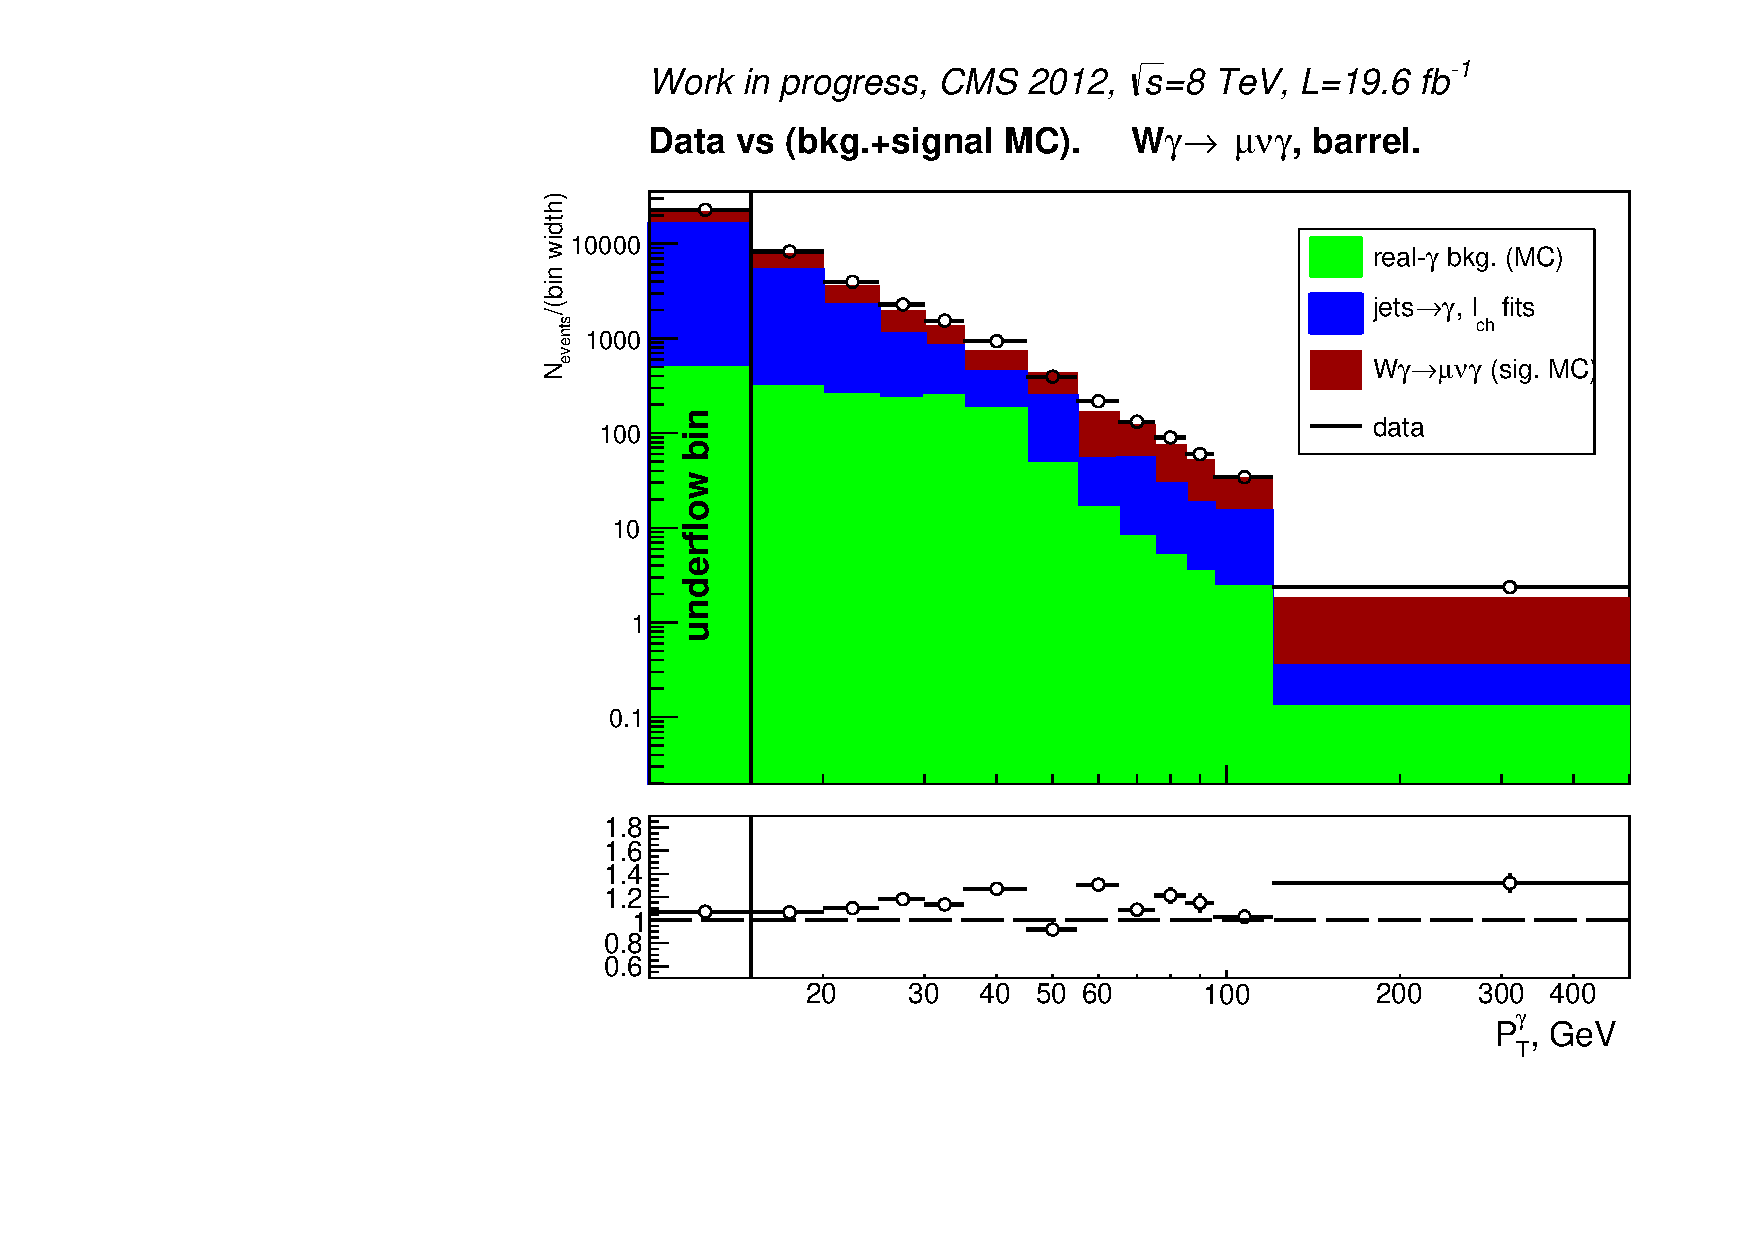
\includegraphics[width=0.45\textwidth]{../figs/figs_v11/MUON_WGamma/PrepareYields/c_DATAvsBkgPlusSigMCc_MUON_WGamma_TEMPL_CHISO_UNblind__Barrel__phoEt.pdf}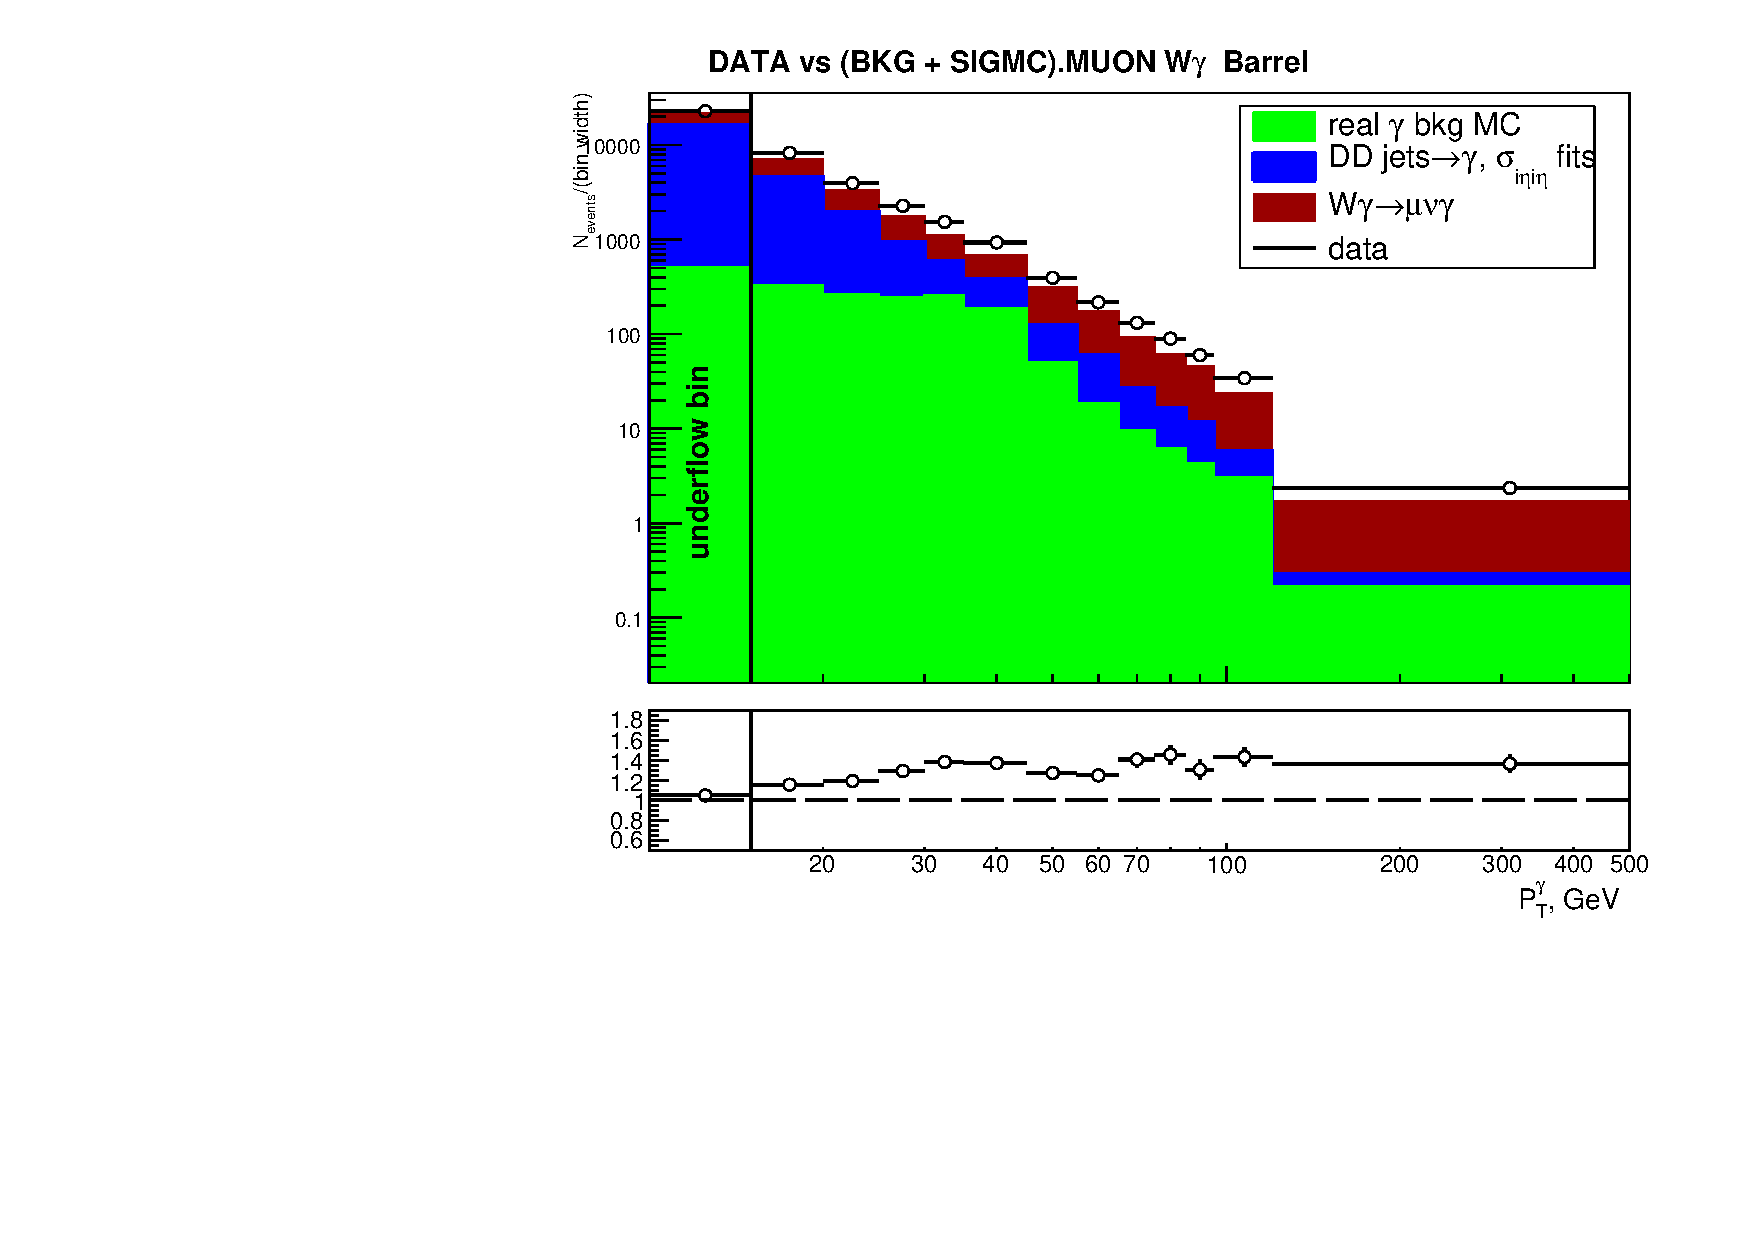
\includegraphics[width=0.45\textwidth]{../figs/figs_v11/MUON_WGamma/PrepareYields/c_DATAvsBkgPlusSigMCc_MUON_WGamma_TEMPL_SIHIH_UNblind__Barrel__phoEt.pdf}  \\
   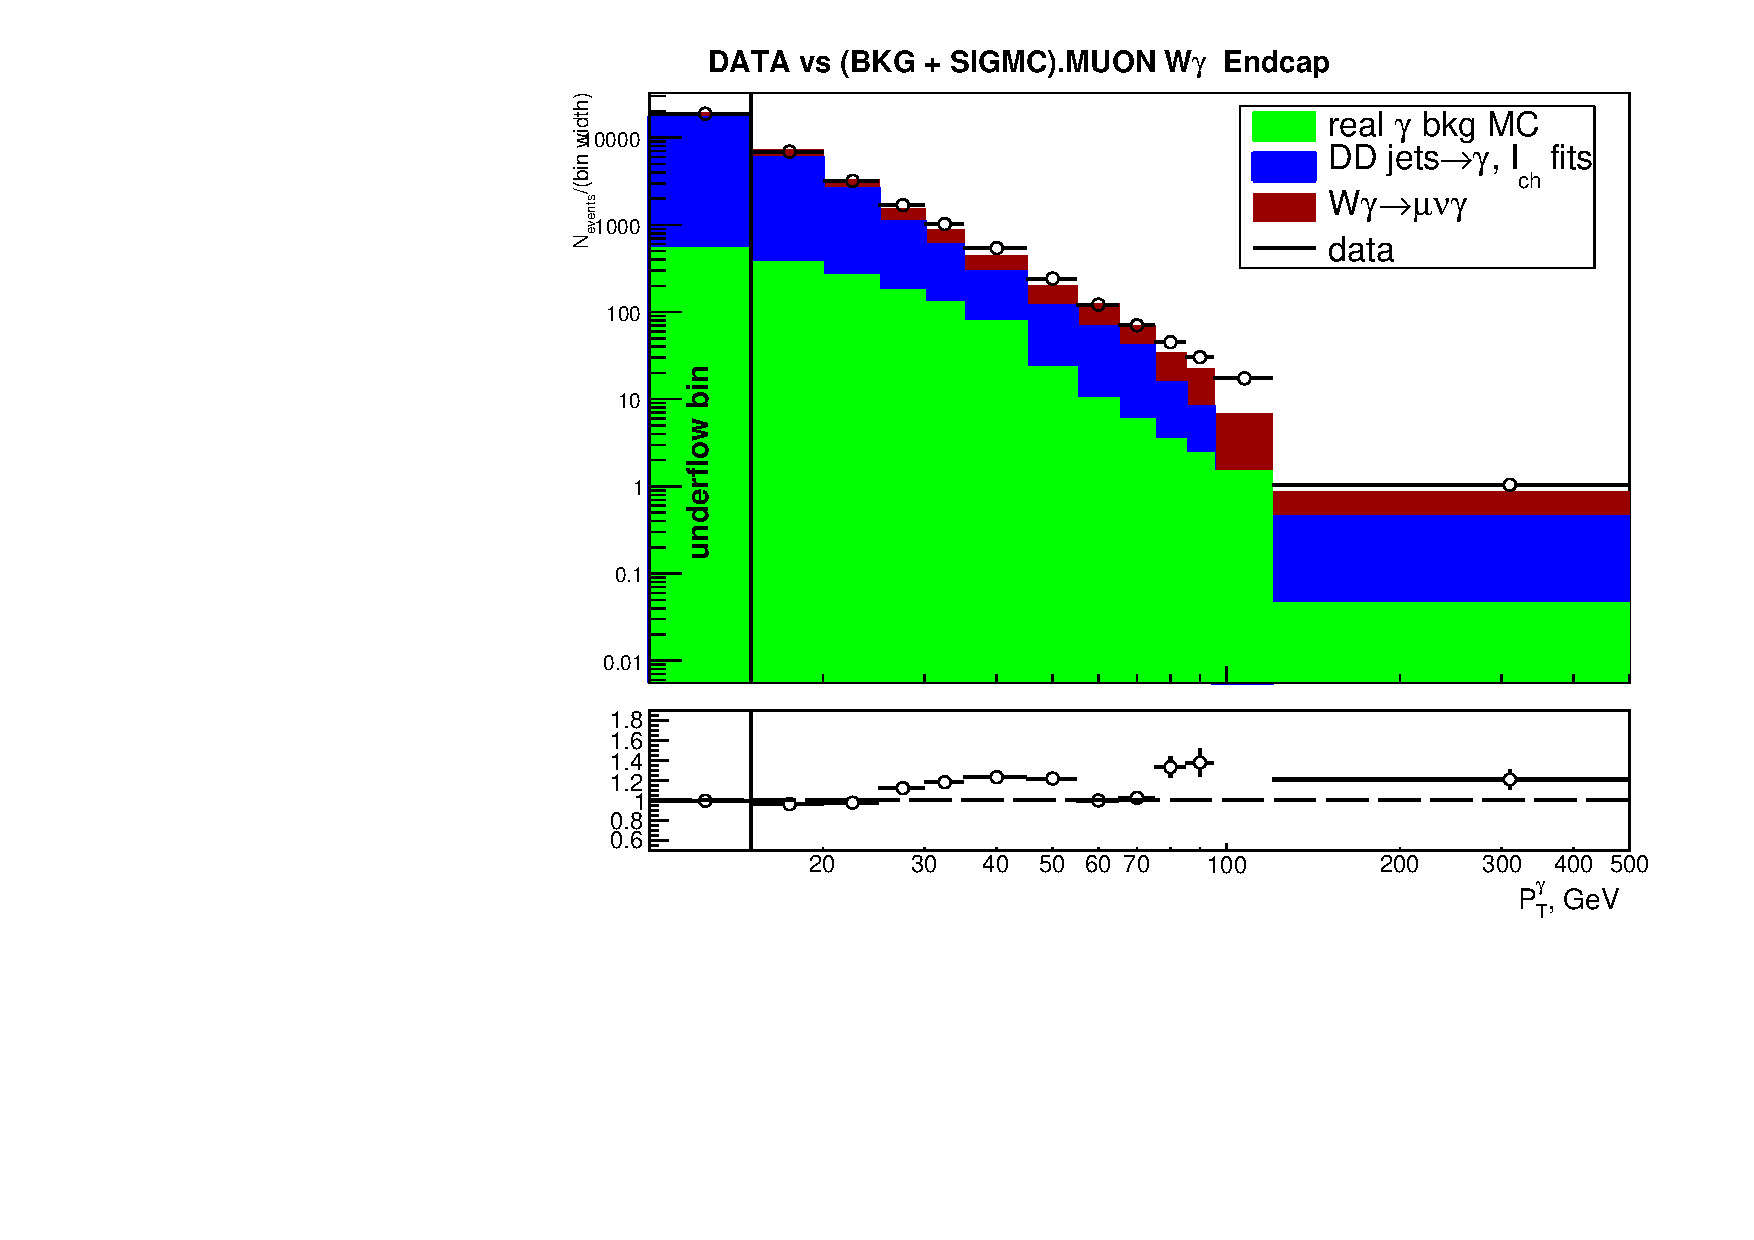
\includegraphics[width=0.45\textwidth]{../figs/figs_v11/MUON_WGamma/PrepareYields/c_DATAvsBkgPlusSigMCc_MUON_WGamma_TEMPL_CHISO_UNblind__Endcap__phoEt.pdf}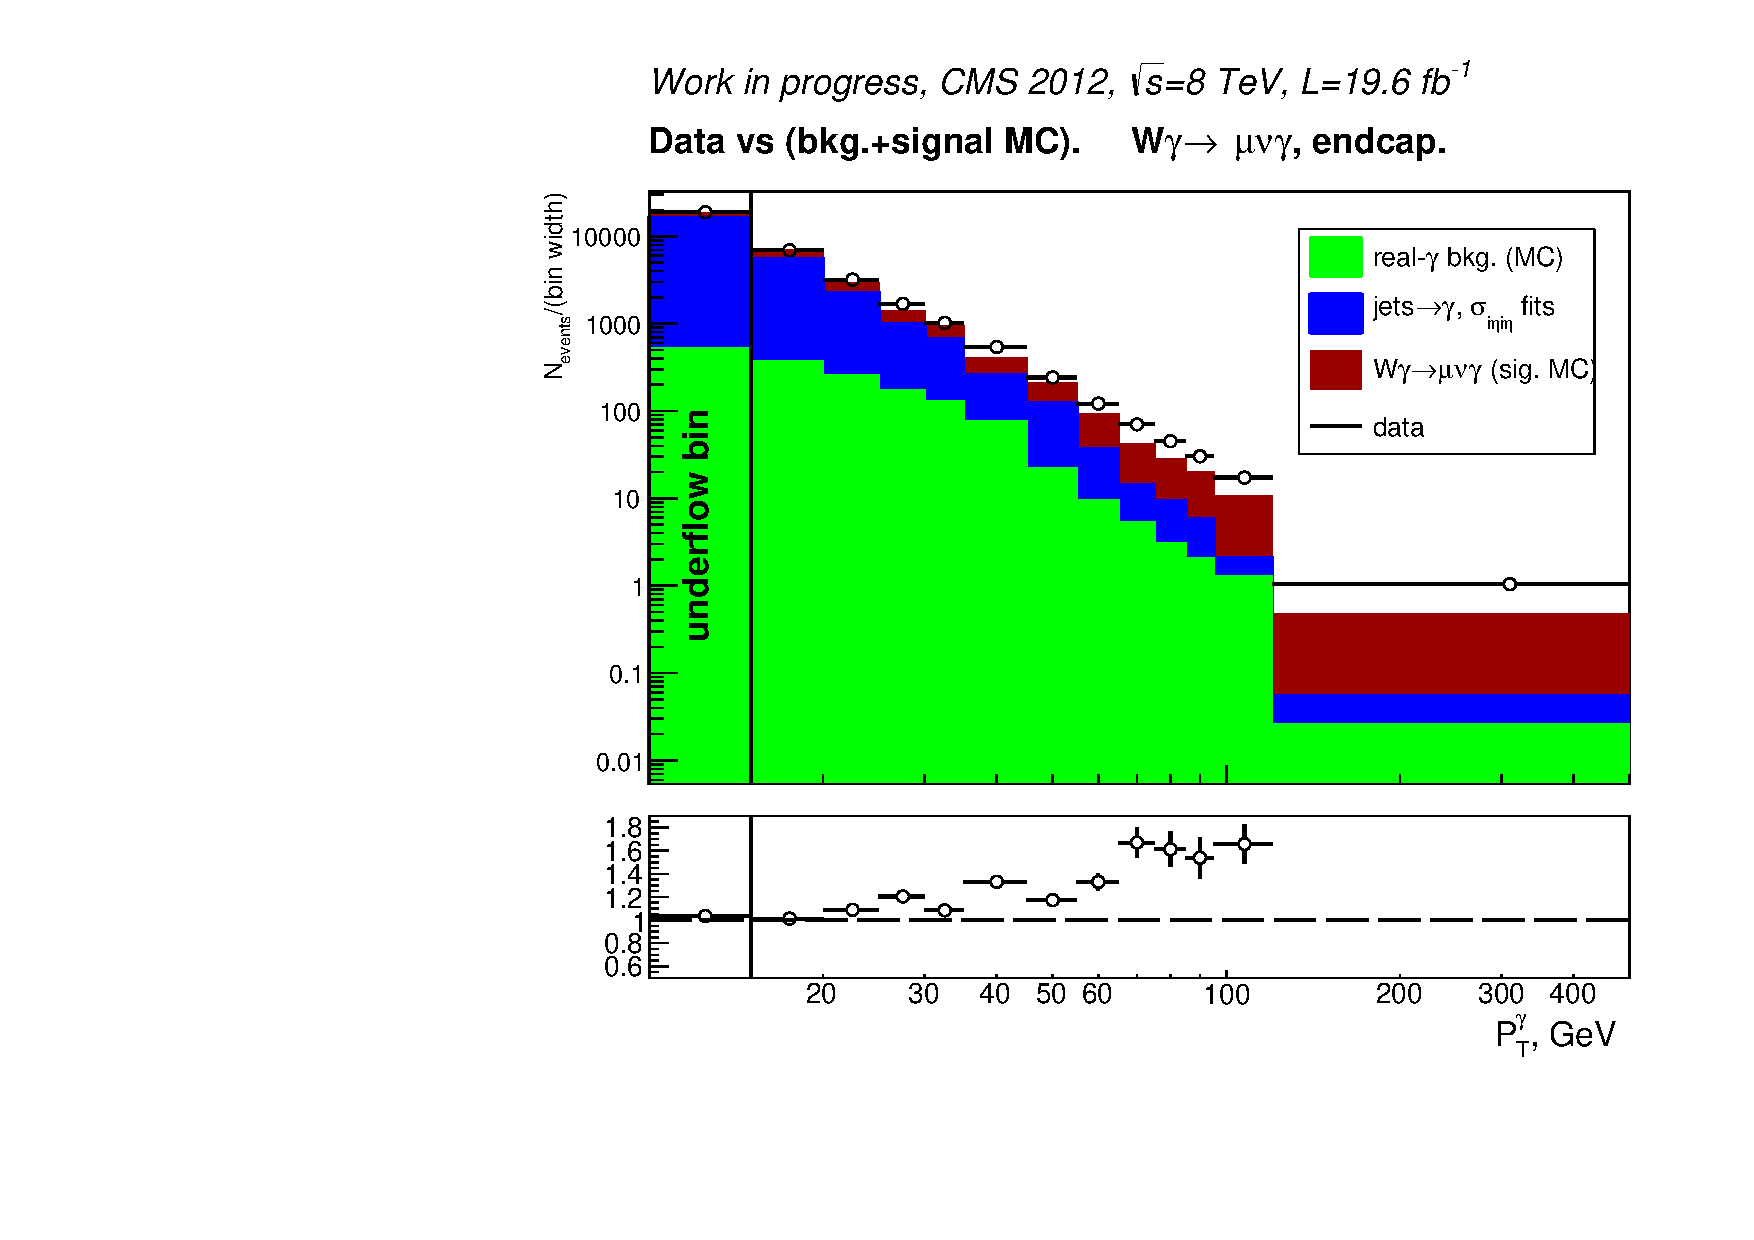
\includegraphics[width=0.45\textwidth]{../figs/figs_v11/MUON_WGamma/PrepareYields/c_DATAvsBkgPlusSigMCc_MUON_WGamma_TEMPL_SIHIH_UNblind__Endcap__phoEt.pdf}  \\
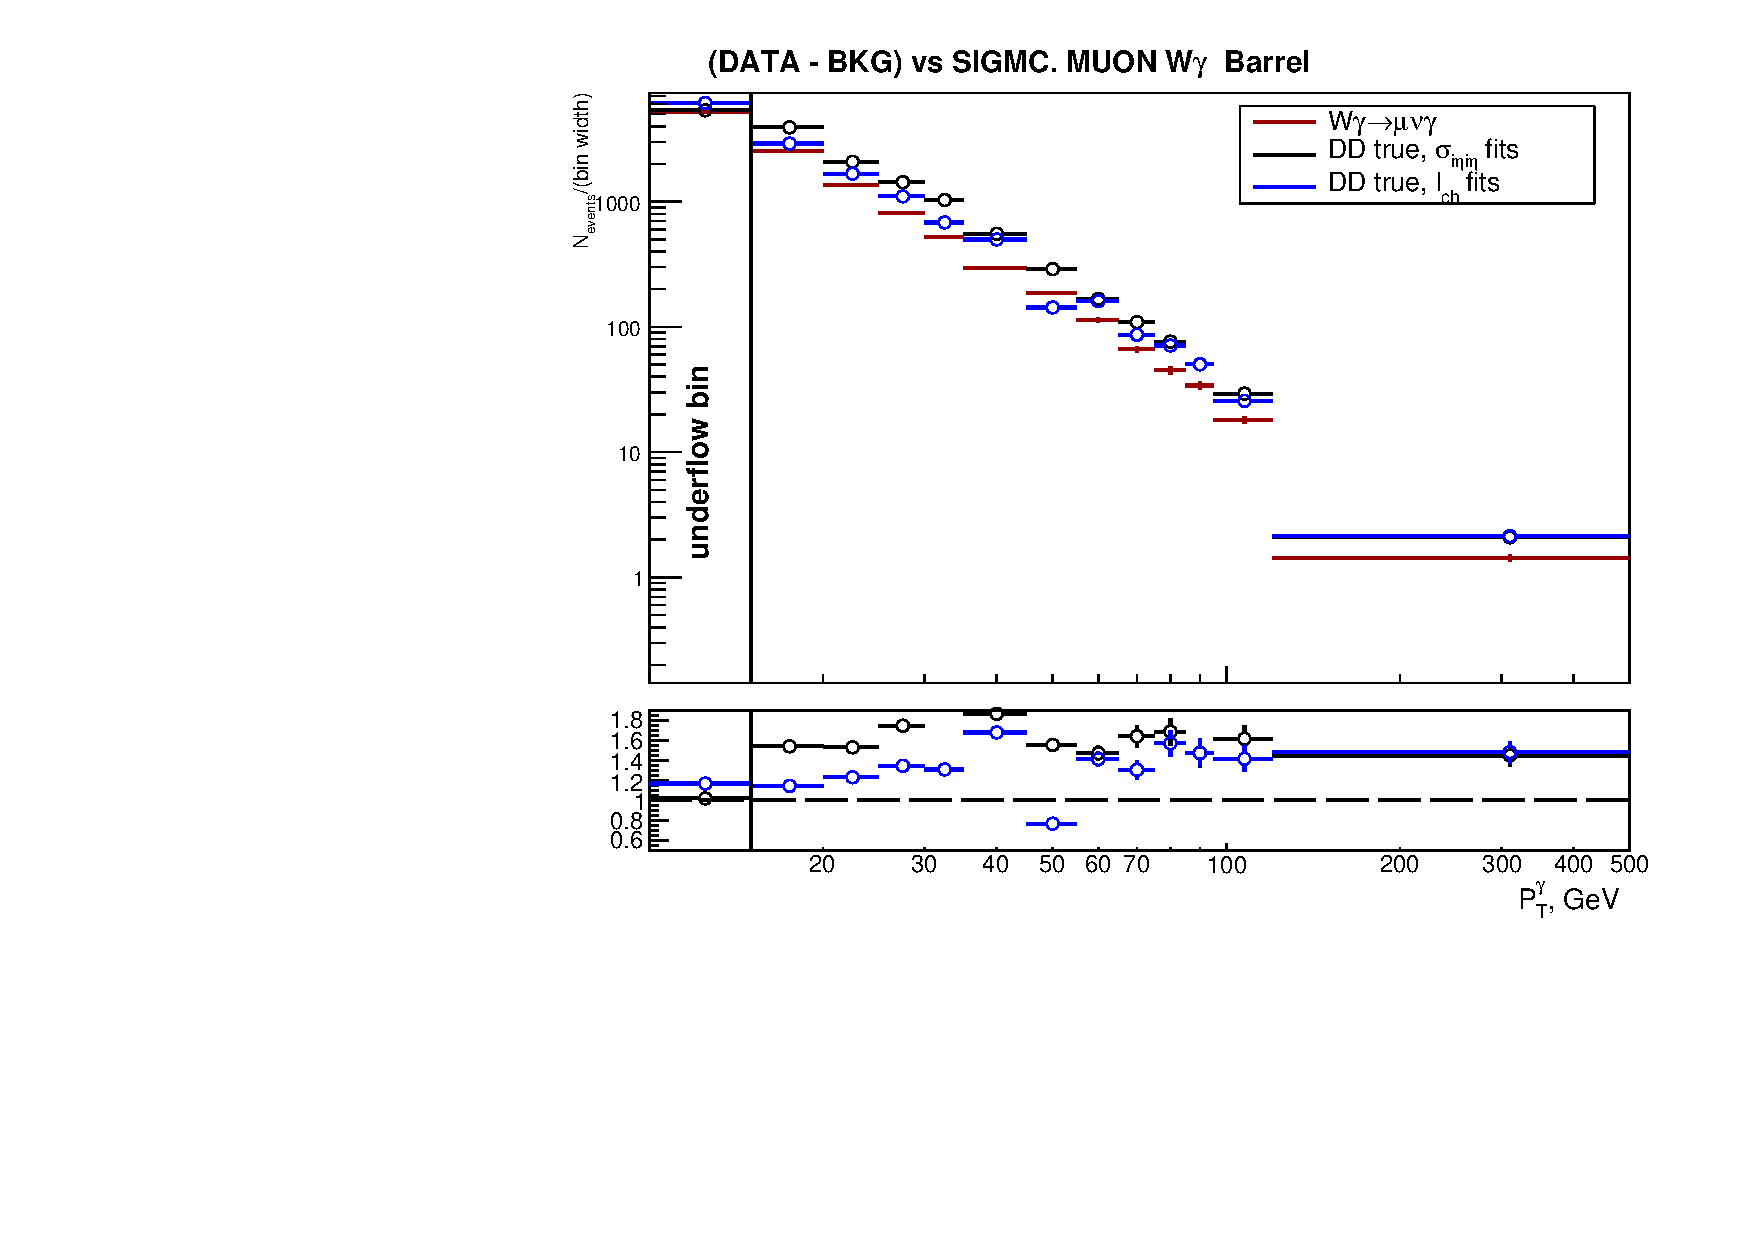
\includegraphics[width=0.45\textwidth]{../figs/figs_v11/MUON_WGamma/PrepareYields/c_BkgSubtrDATAvsSIGMC_c_MUON_WGamma__UNblind__Barrel__phoEt.pdf}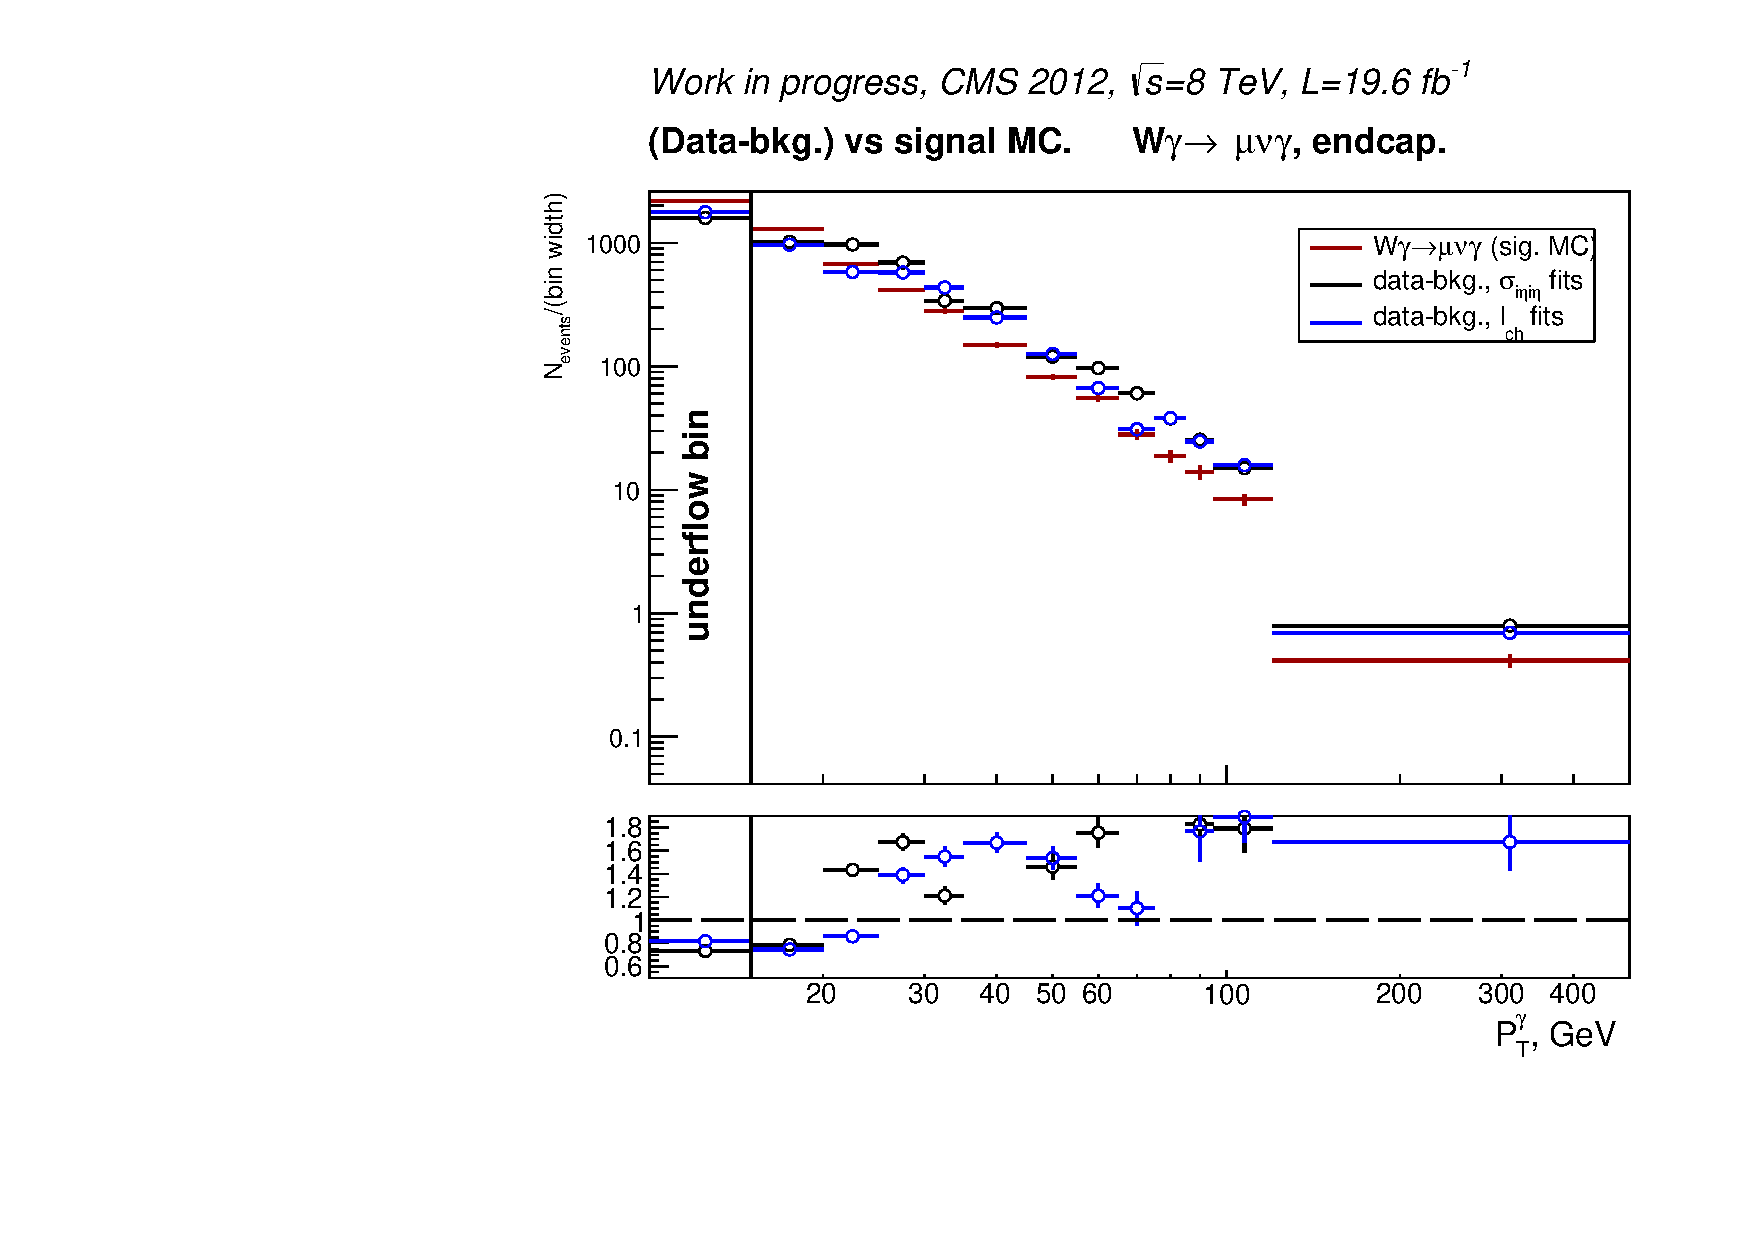
\includegraphics[width=0.45\textwidth]{../figs/figs_v11/MUON_WGamma/PrepareYields/c_BkgSubtrDATAvsSIGMC_c_MUON_WGamma__UNblind__Endcap__phoEt.pdf}\\
  \caption{$P_T^{\gamma}$ spectrum of the $W\gamma$ candidates. $I_{ch}$ vs $\sigma_{i\eta i\eta}$ fit results in the muon channel are compared. Top and middle: data vs fake-$\gamma$ background derived from the template method + real-$\gamma$ background predicted by dedicated MC samples + signal MC, with $I_{ch}$ (left) and $\sigma_{i\eta i\eta}$ (right) used as fit variables in EB (top) and EE (middle). Bottom: data yields after full background subtraction vs signal MC in EB (left) and EE (right).}
  \label{fig:DDvsMC_Wg_Data_MUON}
  \end{center}
\end{figure}

\begin{figure}[htb]
  \begin{center}
   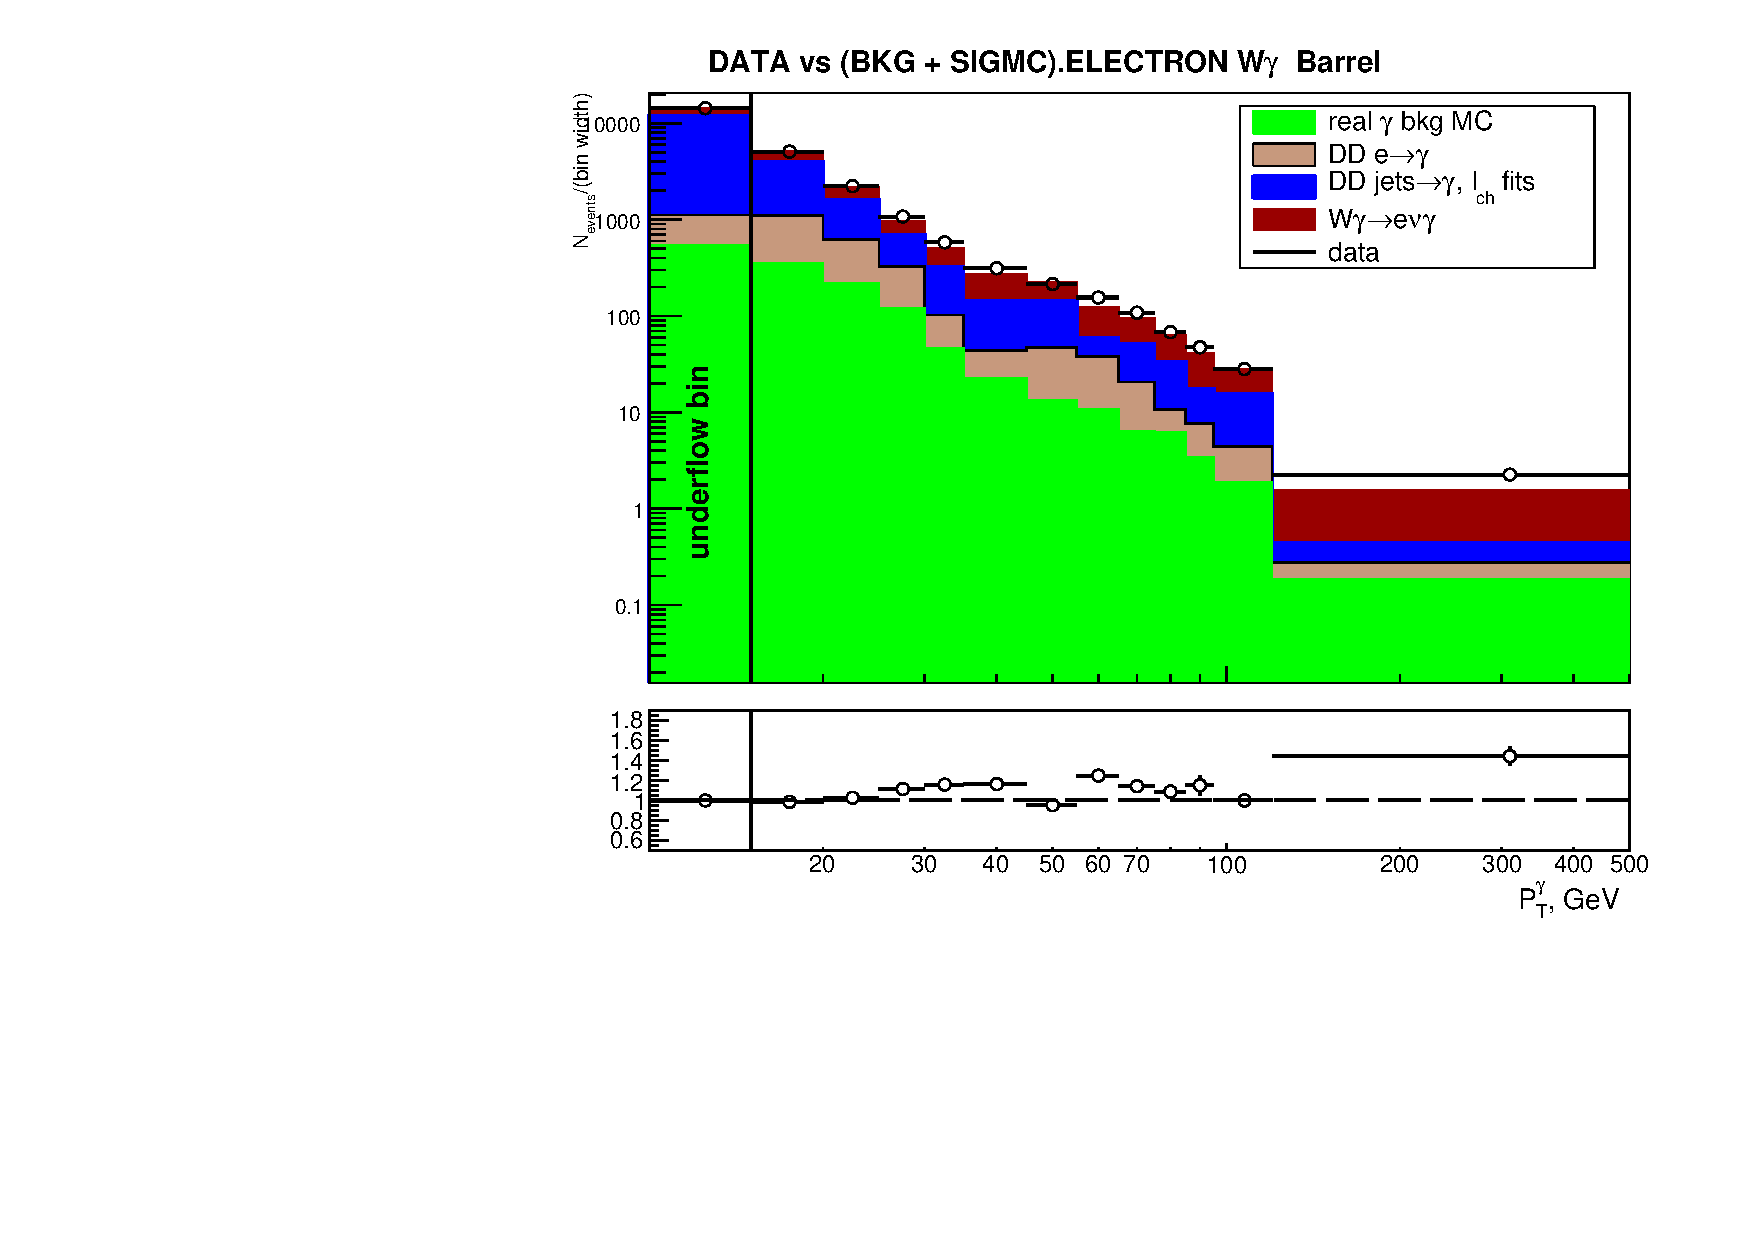
\includegraphics[width=0.45\textwidth]{../figs/figs_v11/ELECTRON_WGamma/PrepareYields/c_DATAvsBkgPlusSigMCc_ELECTRON_WGamma_TEMPL_CHISO_UNblind__Barrel__phoEt.pdf}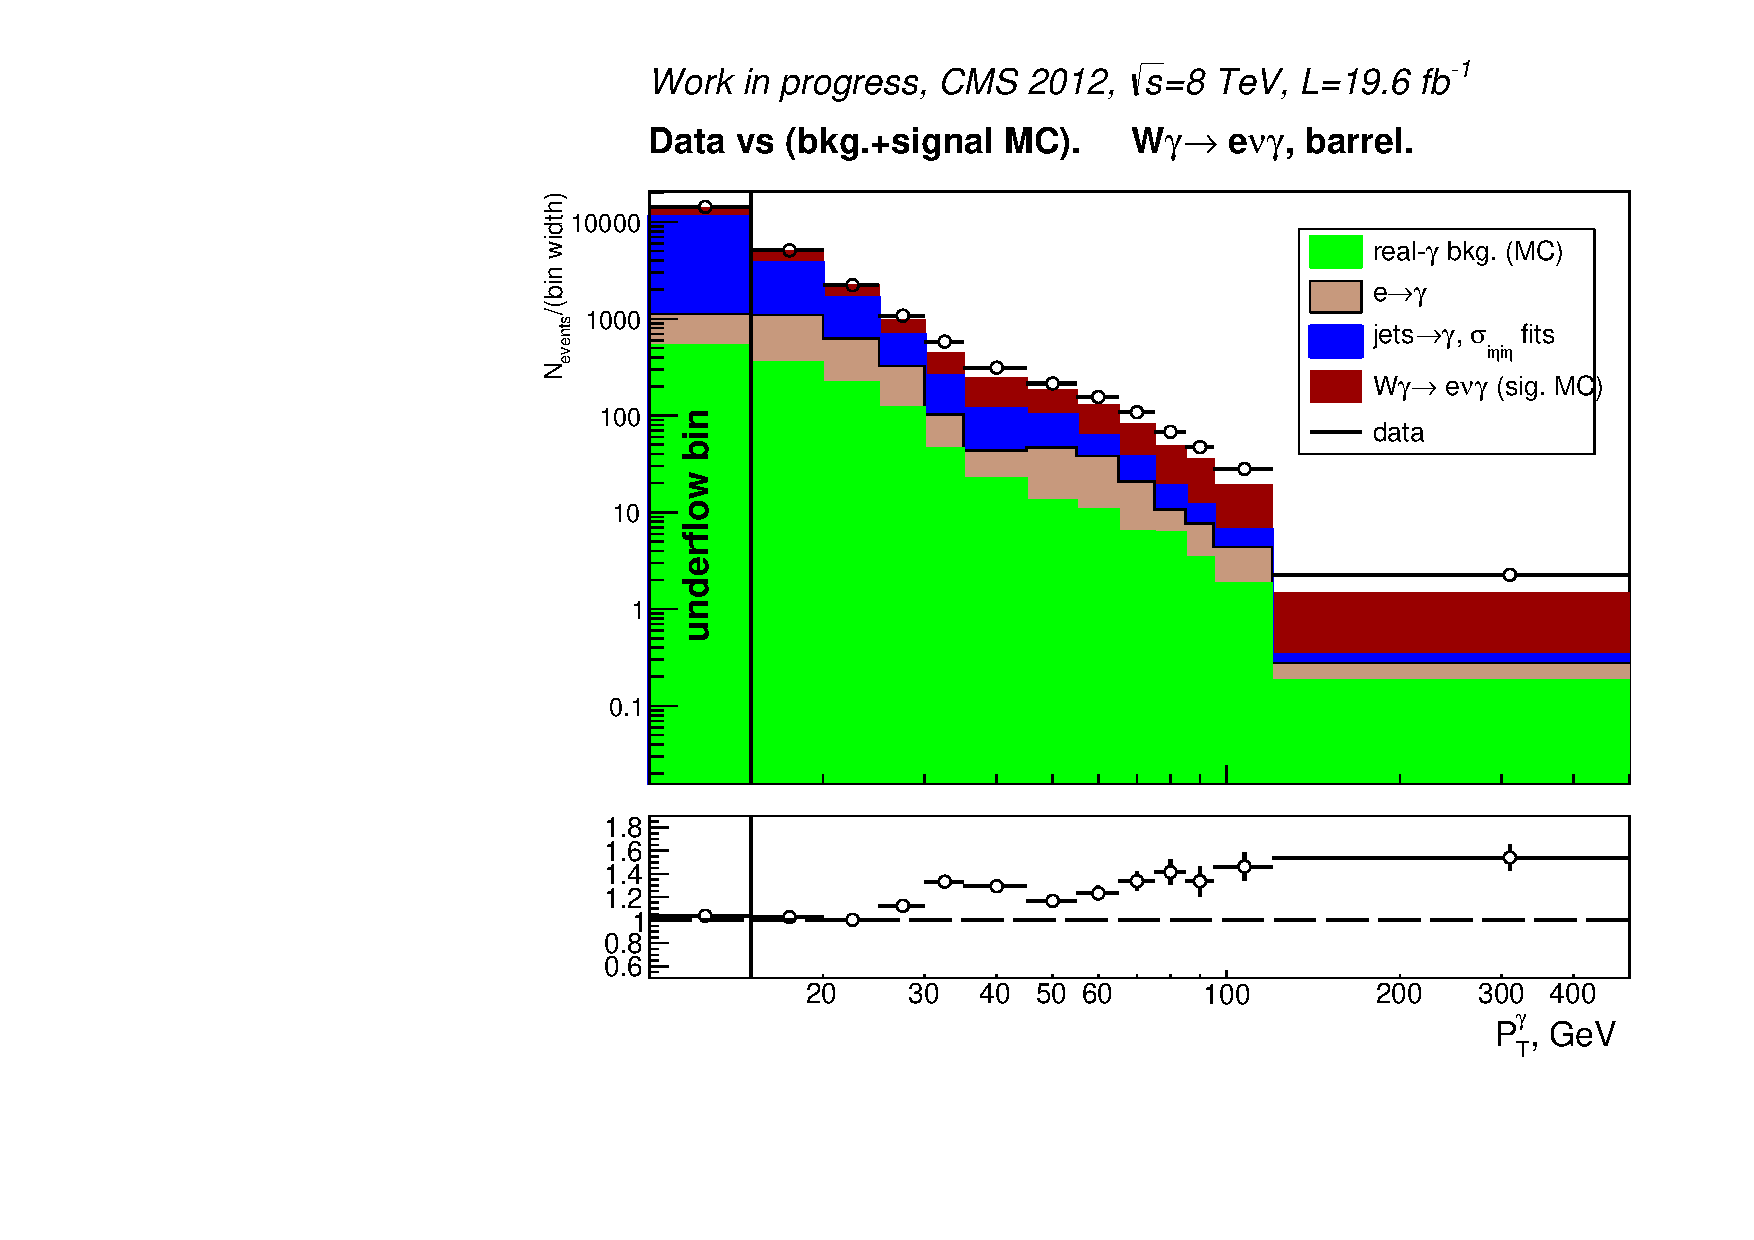
\includegraphics[width=0.45\textwidth]{../figs/figs_v11/ELECTRON_WGamma/PrepareYields/c_DATAvsBkgPlusSigMCc_ELECTRON_WGamma_TEMPL_SIHIH_UNblind__Barrel__phoEt.pdf}  \\
   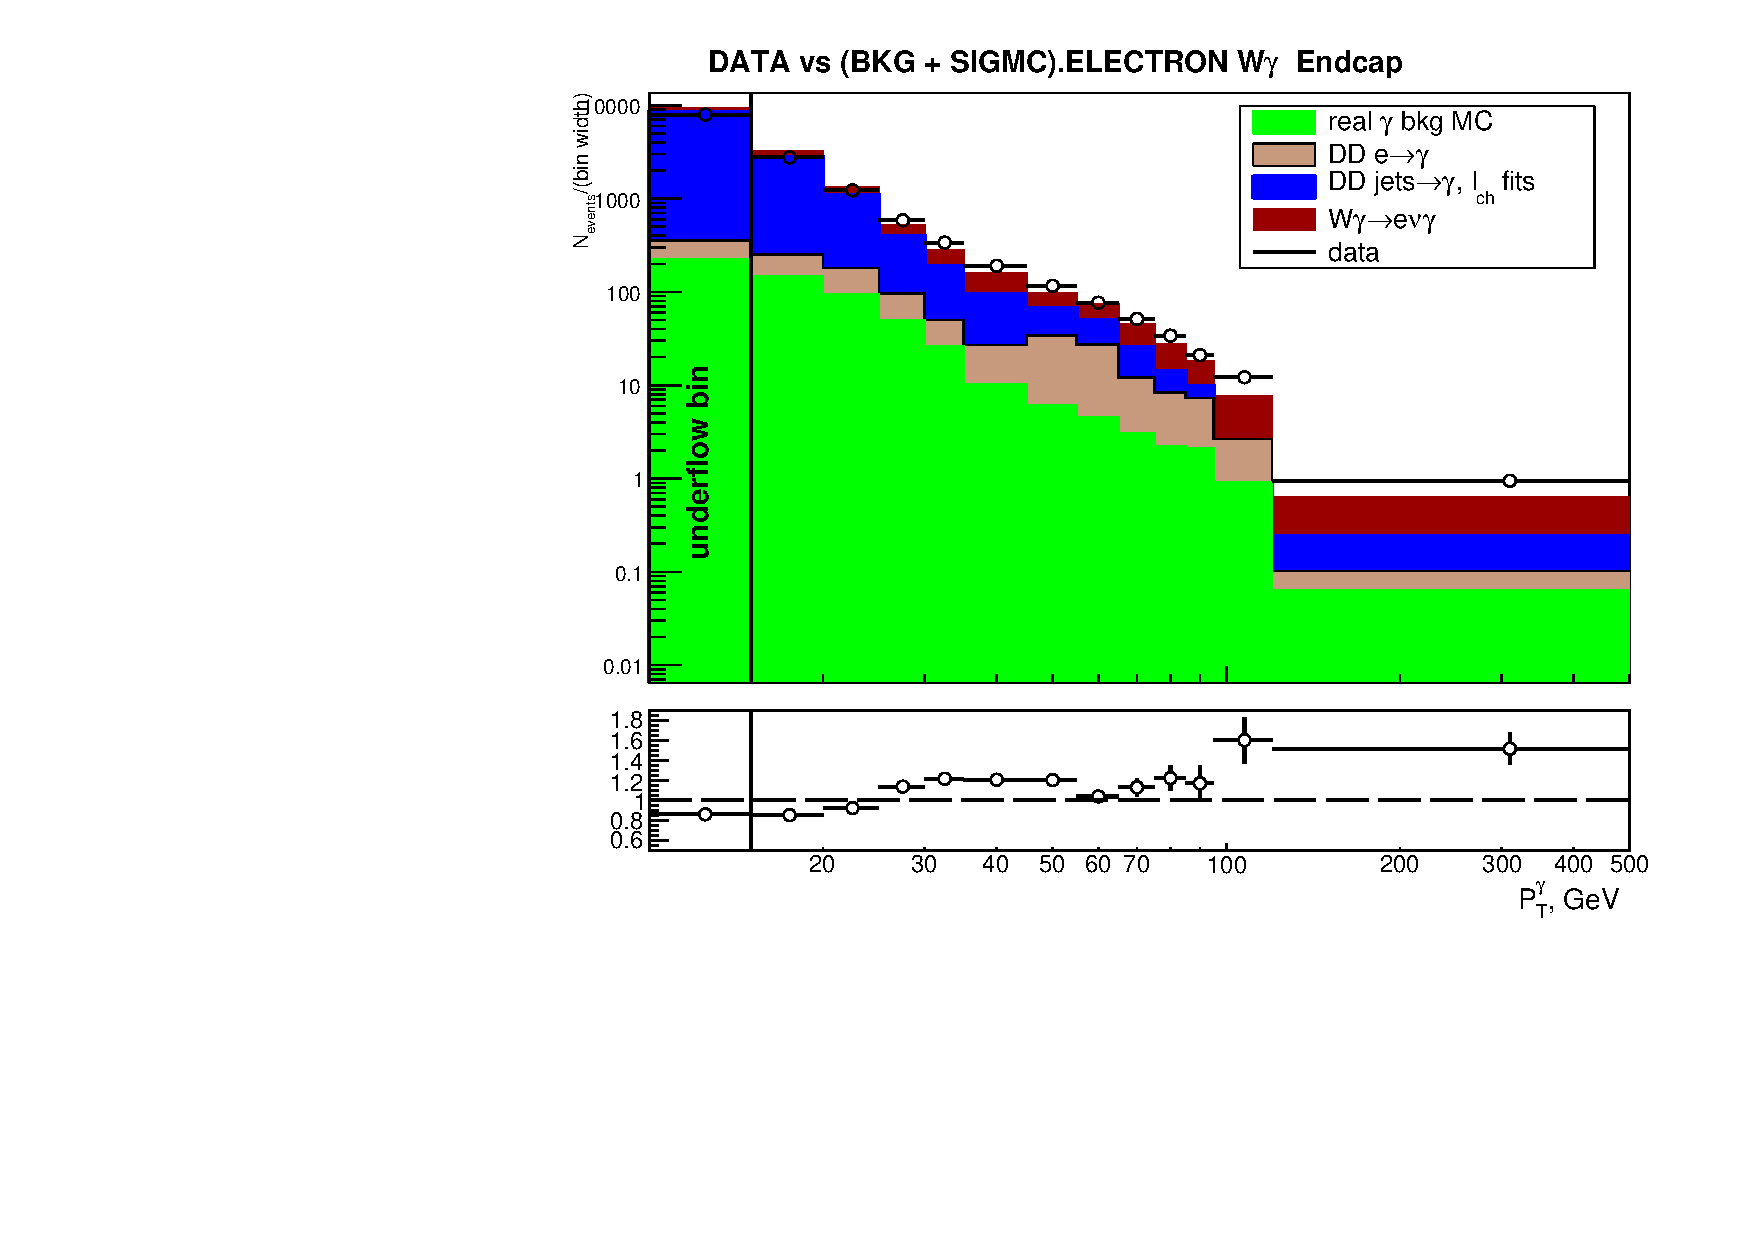
\includegraphics[width=0.45\textwidth]{../figs/figs_v11/ELECTRON_WGamma/PrepareYields/c_DATAvsBkgPlusSigMCc_ELECTRON_WGamma_TEMPL_CHISO_UNblind__Endcap__phoEt.pdf}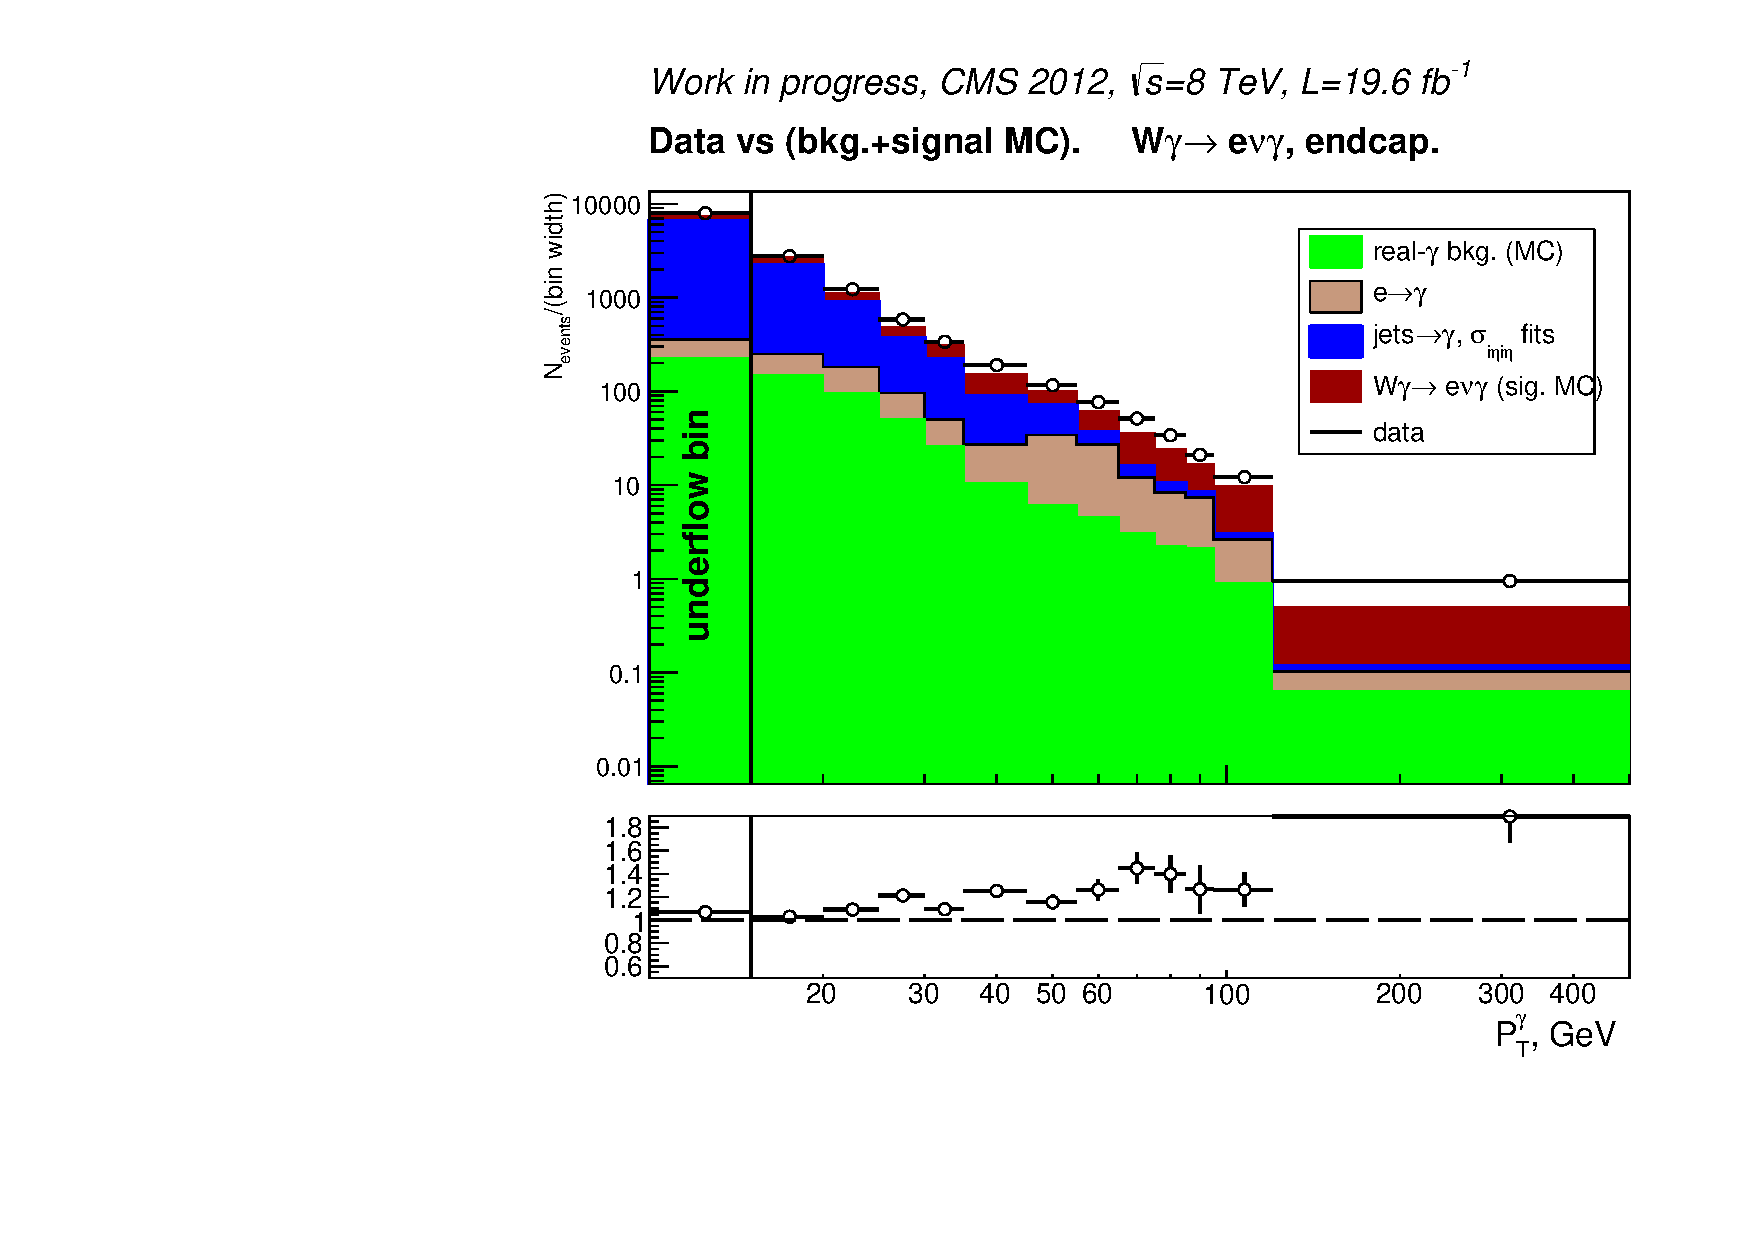
\includegraphics[width=0.45\textwidth]{../figs/figs_v11/ELECTRON_WGamma/PrepareYields/c_DATAvsBkgPlusSigMCc_ELECTRON_WGamma_TEMPL_SIHIH_UNblind__Endcap__phoEt.pdf}  \\
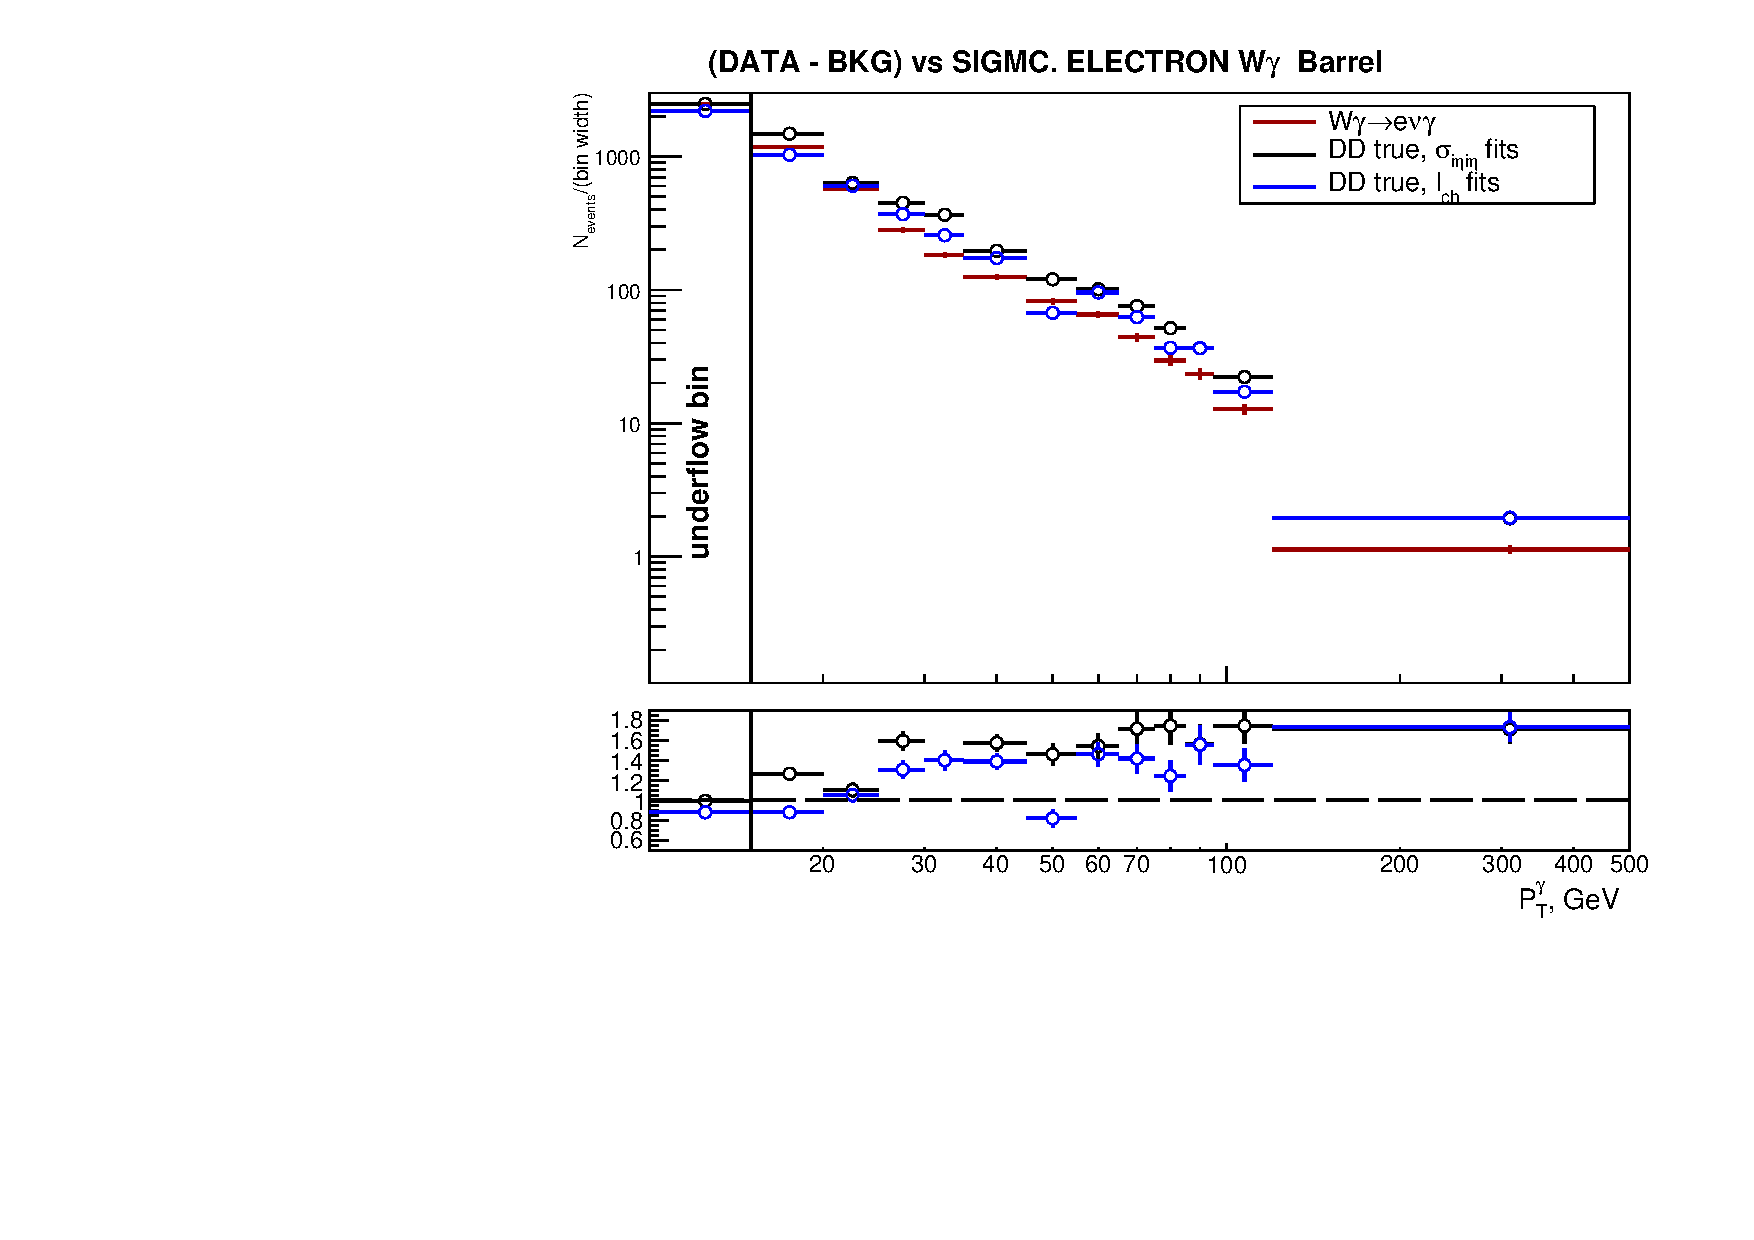
\includegraphics[width=0.45\textwidth]{../figs/figs_v11/ELECTRON_WGamma/PrepareYields/c_BkgSubtrDATAvsSIGMC_c_ELECTRON_WGamma__UNblind__Barrel__phoEt.pdf}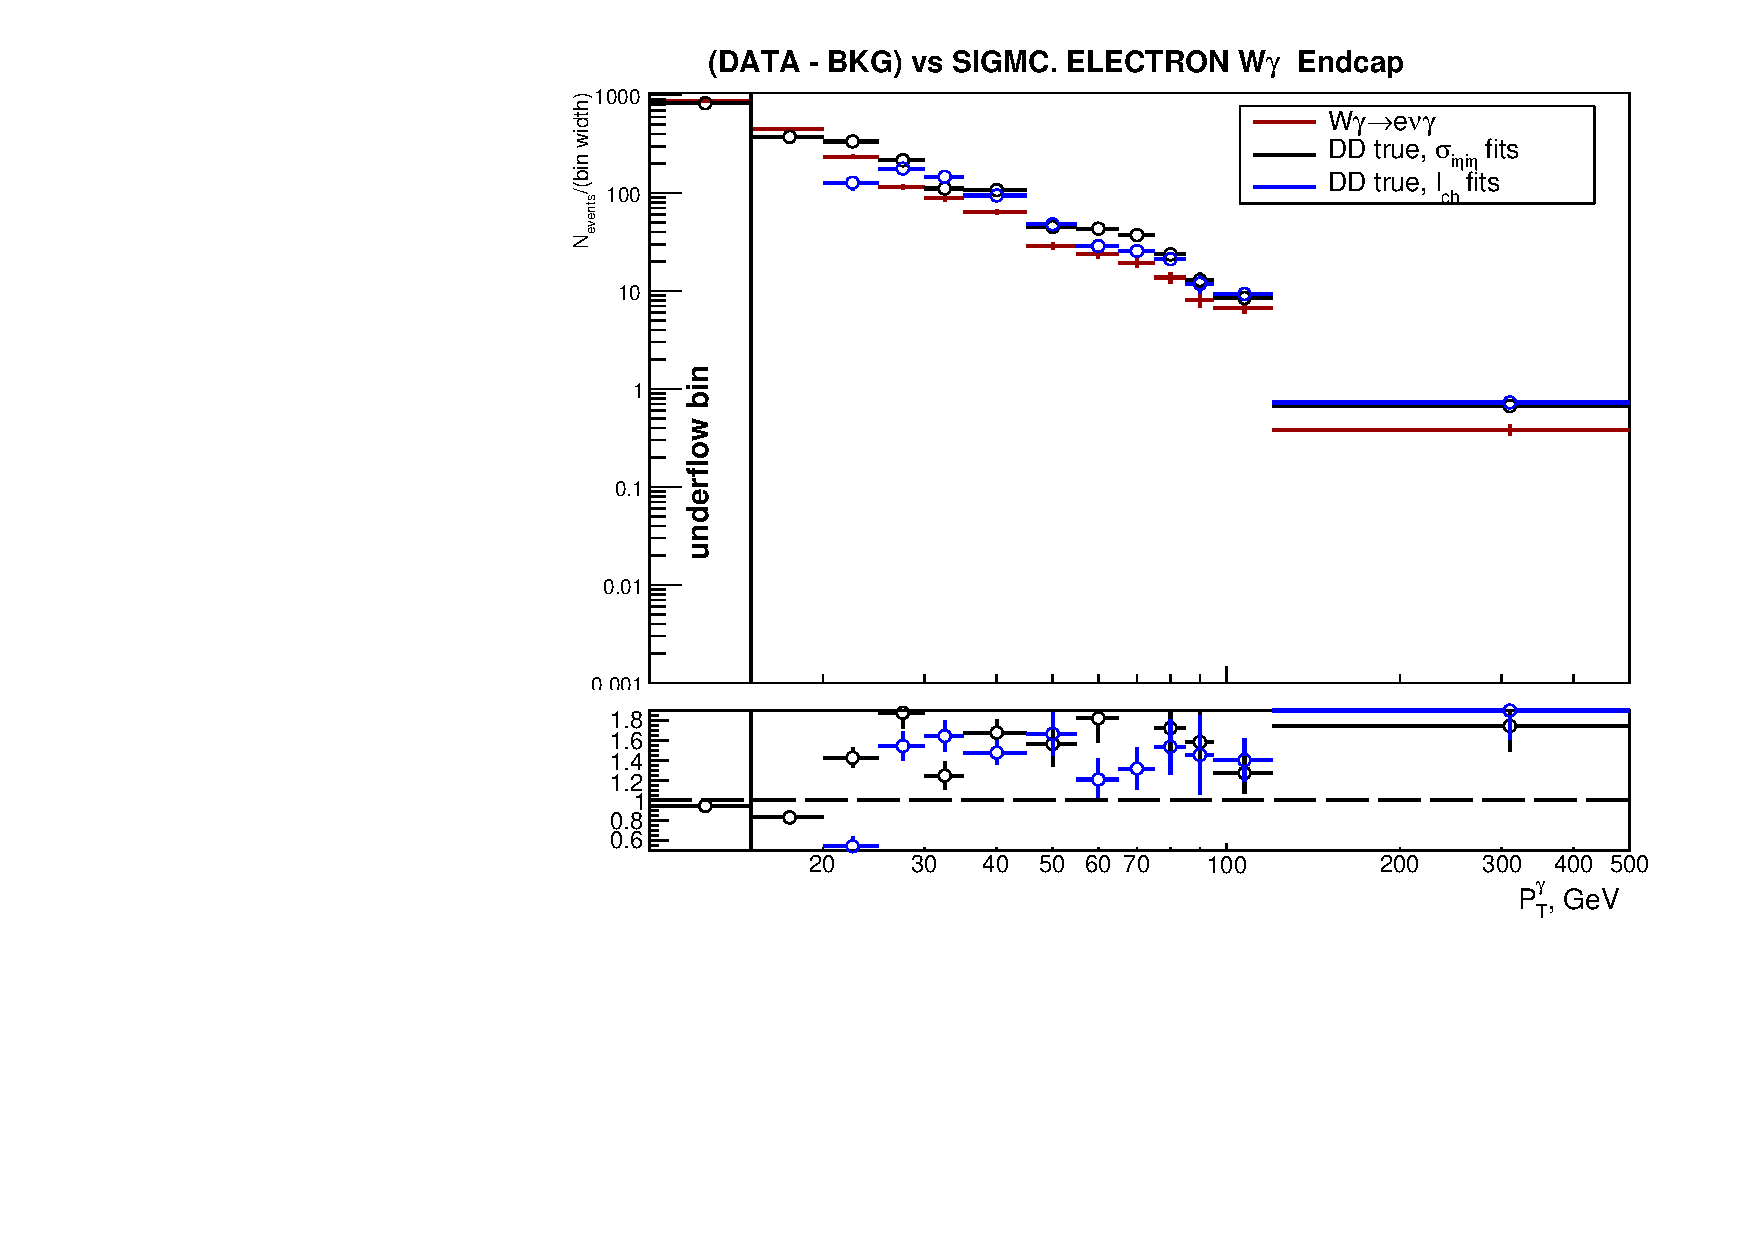
\includegraphics[width=0.45\textwidth]{../figs/figs_v11/ELECTRON_WGamma/PrepareYields/c_BkgSubtrDATAvsSIGMC_c_ELECTRON_WGamma__UNblind__Endcap__phoEt.pdf}\\
  \caption{$P_T^{\gamma}$ spectrum of the $W\gamma$ candidates. $I_{ch}$ vs $\sigma_{i\eta i\eta}$ fit results in the electron channel are compared. Top and middle: data vs fake-$\gamma$ background derived from the template method + real-$\gamma$ background predicted by dedicated MC samples + signal MC, with $I_{ch}$ (left) and $\sigma_{i\eta i\eta}$ (right) used as fit variables in EB (top) and EE (middle). Bottom: data yields after full background subtraction vs signal MC in EB (left) and EE (right).}
  \label{fig:DDvsMC_Wg_Data_ELECTRON}
  \end{center}
\end{figure}

\clearpage

\begin{table}[h]
  \scriptsize
  \begin{center}
  \caption{The $W\gamma$ yields in the muon channel, including selected data yields, jets$\rightarrow\gamma$ and real-$\gamma$ background estimates, yieds after the background subtraction (``data-bkg''), and signal $W\gamma$ yields predicted by MC (``signal MC'').}
  \begin{tabular}{|c|c|c|c|c|c|c|}
  \hline
                  &        &                 &                            &                   &           &   \\ 
    $P_T^{\gamma}$, & data   &  \multicolumn{3}{|c|}{background estimates}                      &  data-bkg & signal      \\ 
    GeV           & yields & \multicolumn{2}{|c|}{jets$\rightarrow\gamma$} & MC real-$\gamma$ &           & MC \\ 
                  &        & $I_{ch}^{\gamma$ & $\sigma_{i\eta i\eta}^{\gamma}$  &                  &           &   \\ \hline
\multicolumn{7}{|c|}{barrel photons}\\ \hline
10-15 & 114047$\pm$338 & 79833$\pm$251 & 77612$\pm$322 & 2453$\pm$46 & 26867$\pm$385 & 26251$\pm$240 \\ \hline 
15-20 & 41411$\pm$203 & 21434$\pm$150 & 24543$\pm$143 & 1566$\pm$34 & 19642$\pm$245 & 12707$\pm$164 \\ \hline 
20-25 & 19801$\pm$141 & 8466$\pm$101 & 9878$\pm$78 & 1283$\pm$31 & 10446$\pm$168 & 6793$\pm$120 \\ \hline 
25-30 & 11409$\pm$107 & 3509$\pm$68 & 4402$\pm$46 & 1180$\pm$27 & 7180$\pm$123 & 4087$\pm$93 \\ \hline 
30-35 & 7717$\pm$88 & 1687$\pm$49 & 2944$\pm$40 & 1253$\pm$27 & 5181$\pm$99 & 2604$\pm$75 \\ \hline 
35-45 & 9339$\pm$97 & 1947$\pm$56 & 2540$\pm$33 & 1840$\pm$33 & 5587$\pm$114 & 2971$\pm$80 \\ \hline 
45-55 & 3950$\pm$63 & 731$\pm$40 & 1964$\pm$40 & 477$\pm$18 & 2923$\pm$75 & 1861$\pm$63 \\ \hline 
55-65 & 2172$\pm$47 & 415$\pm$25 & 363$\pm$11 & 164$\pm$12 & 1694$\pm$50 & 1135$\pm$50 \\ \hline 
65-75 & 1320$\pm$36 & 177$\pm$17 & 466$\pm$19 & 81$\pm$8 & 1106$\pm$39 & 664$\pm$38 \\ \hline 
75-85 & 899$\pm$30 & 103$\pm$13 & 238$\pm$16 & 51$\pm$7 & 773$\pm$32 & 452$\pm$31 \\ \hline 
85-95 & 600$\pm$24 & 76$\pm$11 & 146$\pm$11 & 34$\pm$6 & 510$\pm$26 & 341$\pm$27 \\ \hline 
95-120 & 856$\pm$29 & 67$\pm$11 & 319$\pm$25 & 60$\pm$9 & 750$\pm$31 & 454$\pm$31 \\ \hline 
120-500 & 897$\pm$30 & 28$\pm$7 & 83$\pm$7 & 50$\pm$8 & 825$\pm$31 & 547$\pm$34 \\ \hline 
\multicolumn{7}{|c|}{endcap photons}\\ \hline
10-15 & 94370$\pm$307 & 77649$\pm$215 & 81161$\pm$426 & 2632$\pm$41 & 7937$\pm$306 & 10823$\pm$154 \\ \hline 
15-20 & 34643$\pm$186 & 25902$\pm$142 & 27661$\pm$184 & 1835$\pm$34 & 5089$\pm$213 & 6474$\pm$120 \\ \hline 
20-25 & 15988$\pm$126 & 10018$\pm$93 & 11659$\pm$102 & 1294$\pm$29 & 4842$\pm$138 & 3377$\pm$86 \\ \hline 
25-30 & 8429$\pm$92 & 4061$\pm$58 & 4558$\pm$51 & 871$\pm$23 & 3460$\pm$98 & 2068$\pm$67 \\ \hline 
30-35 & 5110$\pm$71 & 2669$\pm$54 & 2268$\pm$32 & 641$\pm$19 & 1700$\pm$81 & 1404$\pm$56 \\ \hline 
35-45 & 5414$\pm$74 & 1807$\pm$44 & 2113$\pm$29 & 771$\pm$22 & 2957$\pm$83 & 1489$\pm$57 \\ \hline 
45-55 & 2422$\pm$49 & 1025$\pm$50 & 936$\pm$19 & 222$\pm$13 & 1196$\pm$68 & 819$\pm$43 \\ \hline 
55-65 & 1217$\pm$35 & 270$\pm$19 & 564$\pm$16 & 94$\pm$9 & 966$\pm$36 & 551$\pm$35 \\ \hline 
65-75 & 703$\pm$27 & 87$\pm$11 & 346$\pm$13 & 54$\pm$7 & 604$\pm$28 & 280$\pm$25 \\ \hline 
75-85 & 451$\pm$21 & 63$\pm$9 & 117$\pm$6 & 30$\pm$5 & 379$\pm$22 & 186$\pm$20 \\ \hline 
85-95 & 303$\pm$17 & 37$\pm$7 & 56$\pm$4 & 21$\pm$5 & 255$\pm$18 & 139$\pm$18 \\ \hline 
95-120 & 433$\pm$21 & 20$\pm$5 & -81$\pm$5 & 32$\pm$6 & 374$\pm$21 & 209$\pm$22 \\ \hline 
120-500 & 396$\pm$20 & 11$\pm$4 & 153$\pm$12 & 10$\pm$2 & 302$\pm$18 & 157$\pm$19 \\ \hline 
  \end{tabular}
  \label{tab:yields_Wg_to_munu_}
  \end{center}
\end{table}

\clearpage

\begin{table}[h]
  \scriptsize
  \begin{center}
  \caption{The $W\gamma$ yields in the electron channel, including selected data yields, jets$\rightarrow\gamma$, $e\rightarrow\gamma$ and real-$\gamma$ background estimates, yieds after the background subtraction (``data-bkg''), and signal $W\gamma$ yields predicted by MC (``signal MC'').}
  \begin{tabular}{|c|c|c|c|c|c|c|c|}
  \hline
                  &        &                 &                            &     &              &           &   \\ 
    $P_T^{\gamma}$, & data   &  \multicolumn{4}{|c|}{background estimates}                      &  data-bkg & signal      \\ 
    GeV           & yields & \multicolumn{2}{|c|}{jets$\rightarrow\gamma$} & $e\rightarrow\gamma$ & MC real-$\gamma$ &           & MC \\ 
                  &        & $I_{ch}^{\gamma$ & $\sigma_{i\eta i\eta}^{\gamma}$  &  &                &           &   \\ \hline

\multicolumn{8}{|c|}{barrel photons}\\ \hline
10-15 & 71649$\pm$268 & 51004$\pm$200 & 53577$\pm$266 & 2923$\pm$80 & 2688$\pm$41 & 12425$\pm$316 & 12480$\pm$164 \\ \hline
15-20 & 25455$\pm$160 & 13487$\pm$118 & 14474$\pm$110 & 3715$\pm$178 & 1779$\pm$32 & 7422$\pm$262 & 5858$\pm$110 \\ \hline
20-25 & 11130$\pm$105 & 5112$\pm$78 & 4846$\pm$55 & 2023$\pm$137 & 1101$\pm$25 & 3168$\pm$186 & 2869$\pm$77 \\ \hline
25-30 & 5388$\pm$73 & 1748$\pm$47 & 1790$\pm$29 & 1031$\pm$72 & 603$\pm$18 & 2251$\pm$111 & 1412$\pm$54 \\ \hline
30-35 & 2907$\pm$54 & 752$\pm$32 & 1079$\pm$24 & 286$\pm$33 & 229$\pm$12 & 1831$\pm$68 & 916$\pm$44 \\ \hline
35-45 & 3128$\pm$56 & 735$\pm$34 & 1003$\pm$21 & 215$\pm$27 & 223$\pm$12 & 1965$\pm$70 & 1248$\pm$51 \\ \hline
45-55 & 2147$\pm$46 & 551$\pm$31 & 964$\pm$28 & 335$\pm$37 & 134$\pm$10 & 1200$\pm$65 & 821$\pm$42 \\ \hline
55-65 & 1556$\pm$39 & 228$\pm$19 & 211$\pm$8 & 272$\pm$39 & 108$\pm$9 & 1011$\pm$57 & 654$\pm$37 \\ \hline
65-75 & 1083$\pm$33 & 163$\pm$16 & 300$\pm$15 & 143$\pm$27 & 64$\pm$7 & 757$\pm$44 & 441$\pm$31 \\ \hline
75-85 & 680$\pm$26 & 79$\pm$11 & 224$\pm$15 & 45$\pm$13 & 62$\pm$7 & 516$\pm$31 & 295$\pm$26 \\ \hline
85-95 & 473$\pm$22 & 43$\pm$9 & 99$\pm$9 & 43$\pm$17 & 34$\pm$5 & 366$\pm$29 & 234$\pm$23 \\ \hline
95-120 & 703$\pm$27 & 53$\pm$9 & 274$\pm$24 & 63$\pm$19 & 47$\pm$5 & 555$\pm$34 & 318$\pm$27 \\ \hline
120-500 & 859$\pm$29 & 23$\pm$6 & 61$\pm$6 & 34$\pm$12 & 71$\pm$8 & 735$\pm$33 & 430$\pm$31 \\ \hline
\multicolumn{8}{|c|}{endcap photons}\\ \hline
10-15 & 39746$\pm$199 & 31043$\pm$138 & 40022$\pm$13 & 666$\pm$38 & 1120$\pm$27 & 4130$\pm$204 & 4368$\pm$97 \\ \hline
15-20 & 13818$\pm$118 & 9920$\pm$88 & 12692$\pm$124 & 509$\pm$56 & 744$\pm$21 & 1870$\pm$145 & 2253$\pm$68 \\ \hline
20-25 & 6133$\pm$78 & 3538$\pm$56 & 4558$\pm$63 & 433$\pm$36 & 473$\pm$17 & 1680$\pm$92 & 1177$\pm$49 \\ \hline
25-30 & 2924$\pm$54 & 1358$\pm$34 & 1516$\pm$29 & 229$\pm$24 & 250$\pm$12 & 1079$\pm$62 & 575$\pm$34 \\ \hline
30-35 & 1690$\pm$41 & 850$\pm$31 & 694$\pm$18 & 120$\pm$16 & 130$\pm$9 & 555$\pm$49 & 445$\pm$31 \\ \hline
35-45 & 1905$\pm$44 & 613$\pm$26 & 670$\pm$16 & 167$\pm$19 & 103$\pm$8 & 1071$\pm$51 & 638$\pm$37 \\ \hline
45-55 & 1162$\pm$34 & 377$\pm$30 & 337$\pm$11 & 281$\pm$28 & 61$\pm$6 & 450$\pm$53 & 287$\pm$24 \\ \hline
55-65 & 767$\pm$28 & 98$\pm$12 & 228$\pm$11 & 227$\pm$28 & 46$\pm$6 & 433$\pm$40 & 238$\pm$22 \\ \hline
65-75 & 513$\pm$23 & 40$\pm$8 & 139$\pm$9 & 90$\pm$18 & 31$\pm$4 & 372$\pm$29 & 194$\pm$21 \\ \hline
75-85 & 340$\pm$18 & 22$\pm$6 & 57$\pm$5 & 62$\pm$15 & 22$\pm$5 & 236$\pm$24 & 137$\pm$18 \\ \hline
85-95 & 210$\pm$14 & 11$\pm$4 & 25$\pm$3 & 52$\pm$19 & 21$\pm$3 & 129$\pm$24 & 81$\pm$14 \\ \hline
95-120 & 304$\pm$17 & 8$\pm$3 & -43$\pm$4 & 43$\pm$13 & 23$\pm$5 & 212$\pm$22 & 166$\pm$20 \\ \hline
120-500 & 360$\pm$19 & 5$\pm$3 & 53$\pm$7 & 15$\pm$7 & 24$\pm$4 & 254$\pm$18 & 146$\pm$19 \\ \hline
  \end{tabular}
  \label{tab:yields_Wg_to_enu_}
  \end{center}
\end{table}

\subsection{Cross Checks for the Jets$\rightarrow\gamma$ Background Estimation}
\label{sec:AN_BackSubtr_Closure}

For the first MC closure check, we prepare the pseudodata sample by mixing simulated $W$+jets and $W\gamma$ together to mimic real data. Events in both samples are weighted to the same luminosity $L=$19.6~fb$^{-1}$. Real-$\gamma$ templates are prepared from the $W\gamma$ subsample of the mixture while the fake-$\gamma$ templates are prepared from the $W$+jets subsample. Then fits on this sample of pseudodata are performed and the number of real-$\gamma$ and fake-$\gamma$ events determined from fit are compared to the known numbers of simulated events that went into preparing the mixture. The outcome of this cross check cannot be affected by  the effects of possible wrong normalizations of MC samples and the difference between real-$\gamma$ and fake-$\gamma$ $I_{ch}^{\gamma}$ and $\sigma_{i\eta i\eta}^{\gamma}$ distributions in $W\gamma$/$W$+jets and $Z\gamma$/DY+jets samples, and therefore gives us a cleaner test of other effects. The real-$\gamma$ yields extracted from fits and the $W\gamma$ MC prediction are in agreement within~20\%, however, the fake-$\gamma$ yields extracted from fits have larger discrepancies with $W$+jets MC predictions in certain high $P_T^{\gamma}$ bins where real-$\gamma$ fraction is higher, and a small discreapncy in real-$\gamma$ yields leads to large discrepancies in fake-$\gamma$ yields (App.~\ref{sec:MCclosureCheck}, Fig.~\ref{fig:TrueDDvsMC_MCclosureWjetsPlusWg}-\ref{fig:FakeDDvsMC_MCclosureWjetsPlusWg}).

The second check is more realistic: the $W\gamma$ selection requirements are applied on MC samples $W\gamma$, $W$+jets, $Z\gamma$, $Z$+jets, and $t\bar{t}$+jets, and afterwards these samples and mixed together into the pseudodata sample~I. To prepare templates, $Z\gamma$ and $DY$+jets MC samples are mixed together to constitute a $Z\gamma$-selected pseudodata sample~II which is used the same way as $Z\gamma$-selected dataset is used to prepare templates for the background estimation in the data analysis. Then the pseudodata~I histograms are fitted and the fit results are superimposed with MC predictions same as it is done for the real data. The outcome of this closure check is not affected by the effects of possible wrong normalizations of MC samples but is affected by the effect of the possible difference between real-$\gamma$ and fake-$\gamma$ $I_{ch}^{\gamma}$ and $\sigma_{i\eta i\eta}^{\gamma}$ distributions in $W\gamma$/$W$+jets and $Z\gamma$/DY+jets samples. The results of this closure check show better agreement of pseudodata~I vs estimated background + signal MC than we observe in data, however the disagreement in certain $P_T^{\gamma}$ bins remains significant (App.~\ref{sec:MCclosureCheck}, Fig.~\ref{fig:DATAvsBKGandSIGMC_MCclosure_MUON_B}-\ref{fig:DATAvsBKGandSIGMC_MCclosure_ELECTRON_E}).

In addition to the checks described above, we also perform $Z\gamma$ check on data and MC mixture. $Z\gamma$ check tests the effects of possibly wrong $Z\gamma$ normalization, effects of the merging several $P_T^{\gamma}$ bins, and the bias in the fit machinery, while is not affected by possible differences in $I_{ch}^{\gamma}$ and $\sigma_{i\eta i\eta}^{\gamma}$ distirbutions between $W\gamma$/$W$+jets and $Z\gamma$/DY+jets events. Both $Z\gamma$ data analysis and $Z\gamma$ MC closure check show very good agreement between data and background estimates + signal MC as well as between two methods of the background estimation. The detailed description of the $Z\gamma$ check is available at App.~\ref{sec:ZgCheck}. 

The results of the cross checks show that our main sources of disagreements in Fig.~\ref{fig:DDvsMC_Wg_Data_MUON}-\ref{fig:DDvsMC_Wg_Data_ELECTRON} related to jets$\rightarrow\gamma$ background estimation are differences in $I_{ch}^{\gamma}$ and $\sigma_{i\eta i\eta}^{\gamma}$ distirbutions between $W\gamma$/$W$+jets and $Z\gamma$/DY+jets events, and sometimes there is also an impact from the bias in the fit machinery. Related systematic uncertainties are discussed in Ch.~\ref{sec:Systematics}.

